% Chapter Template

\chapter{Ρομποτική Πλατφόρμα} % Main chapter title


\label{Chapter2} % Change X to a consecutive number; for referencing this chapter elsewhere, use \ref{ChapterX}

%----------------------------------------------------------------------------------------
%	SECTION 1: Monstertruck Robotic Platform
%----------------------------------------------------------------------------------------
\section{Ρομποτική Πλατφόρμα \textit{Monstertruck}}
Η ρομποτική πλατφόρμα \textit{Monstertruck} αποτελεί ένα ρομποτικό όχημα, η ανάπτυξη του οποίου, ξεκίνησε στα πλαίσια της ομάδας P.A.N.D.O.R.A. και ολοκληρώθηκε στα πλαίσια της παρούσας διπλωματικής. Αναπτύχθηκε με σκοπό την χρήση σε εφαρμογές αυτόνομης λειτουργίας, για χαρτογράφηση και εξερεύνηση άγνωστων χώρων και αναζήτηση σημείων ενδιαφέροντος, αλλά και για πειραματισμό με εναλλακτικά μοντέλα κίνησης οχημάτων.

\subsection{Τηλεκατευθυνόμενο Όχημα GroundPounder}
Για την κατασκευή της ρομποτικής πλατφόρμας, χρησιμοποιήθηκε, σαν βάση, το τηλεκατευθυνόμενο όχημα \textit{GroundPounder} της \textit{Redcat Racing}. Ανήκει στην κατηγορία φορτηγών οχημάτων \textit{Monstertruck}, με κλίμακα 1:10 και περιλαμβάνει σκελετό από αλουμίνιο, όπως επίσης, και ρυθμιζόμενες αναρτήσεις. Επιπλέον, περιλαμβάνει σύστημα ανεξάρτητης στρέψης των μπροστινών και πίσω τροχών (\textit{Τετραδιεύθυνση - 4-Wheel-Steering}), σε συνδυασμό με μετάδοση της κίνησης και στους τέσσερις τροχούς (\textit{Τετρακίνηση} ή \textit{4-Wheel-Drive}), προσφέροντας μεγαλύτερη ευελιξία και δυνατότητες, συγκριτικά με τα συμβατικά αυτοκίνητα, που περιλαμβάνουν στρέψη, μόνο, των μπροστινών τροχών(\textit{2-Wheel-Steering}) και κίνηση μόνο των μπροστινών (\textit{Μπροστινοκίνηση - Front-Wheel-Drive}), ή μόνο των πίσω (\textit{Πισωκίνηση - Rear-Wheel-Drive}).

\begin{figure}[!ht]
	\begin{center}
		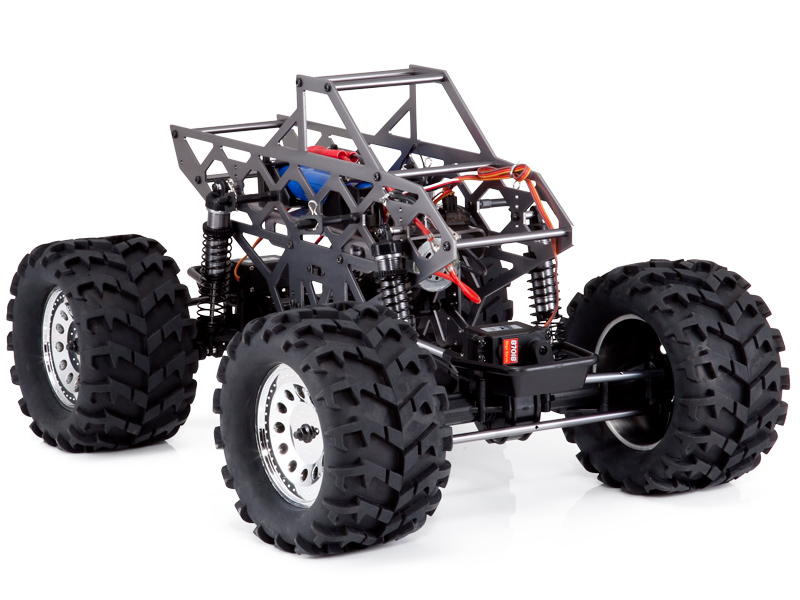
\includegraphics[width=10cm]{Chapters/Chapter2/Figures/groundpounder.jpg}
		\caption{Το τηλεκατευθυνόμενο όχημα \textit{GroundPounder}, της Redcat Racing.}
		\label{fig:groundpounder}
	\end{center}
\end{figure}

\bigskip
\subsection{Σασί Ρομποτικής Πλατφόρμας}
Λόγω, της πληθώρας αισθητήρων, ηλεκτρονικών, καλωδιώσεων κλπ. και του περιορισμένου ελεύθερου χώρου πάνω στο όχημα, κρίθηκε σκόπιμο, αυτό, να επεκταθεί, με πρόσθετους χώρους. Για την λύση του προβλήματος, σχεδιάστηκαν, λοιπόν, και κατασκευάστηκαν, από μέλη της ομάδας \textit{P.A.N.D.O.R.A. 2014-15}, δύο κουτιά, τα οποία προστέθηκαν επάνω στο υπάρχον όχημα, με σκοπό, να περιλάβουν τα επιμέρους εξαρτήματα του ρομπότ.

\begin{figure}[!ht]
	\centering
	\subfloat[To \textit{Κουτί Τροφοδοσίας} της ρομποτικής πλατφόρμας]{
		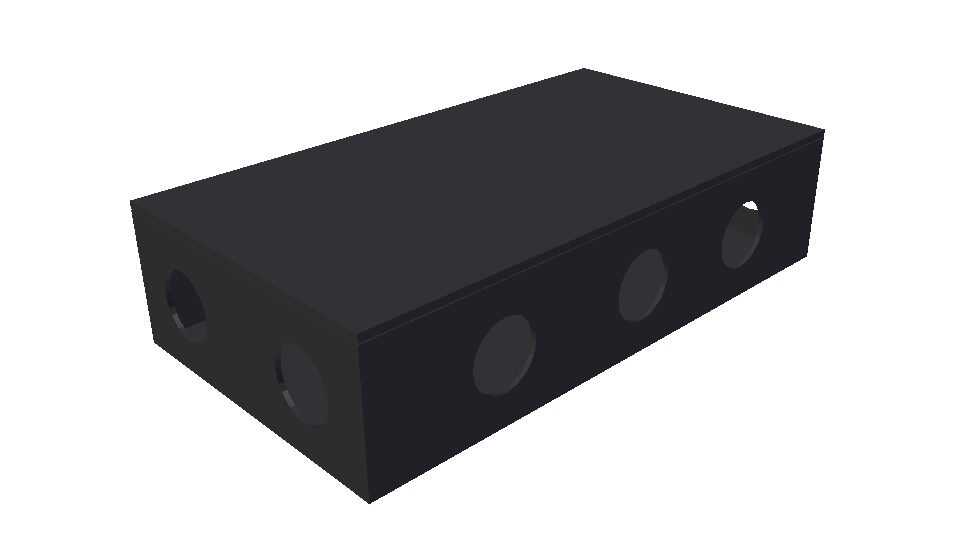
\includegraphics[width=0.45\linewidth]{Chapters/Chapter2/Figures/power_box.png}
		\label{fig:power_box}}
	\subfloat[To \textit{Κουτί Ηλεκτρονικών} της ρομποτικής πλατφόρμας]{
		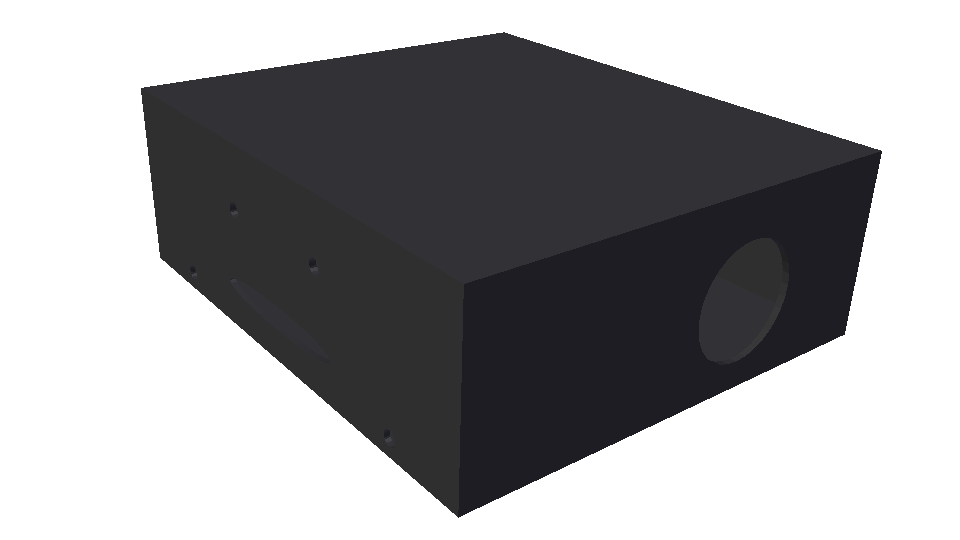
\includegraphics[width=0.45\linewidth]{Chapters/Chapter2/Figures/electronics_box.png}
		\label{fig:electronics_box}}
	\caption{Τα κουτιά του σασί.}
\end{figure}

\bigskip
Το \textit{Κουτί Τροφοδοσίας}, του σασί της ρομποτικής πλατφόρμας, που παρουσιάζεται στο σχήμα \ref{fig:power_box}, έχει διαστάσεις $310mm \times 170mm \times 74mm$, και περιλαμβάνει 10 τρύπες, διαμέτρου 35mm, τοποθετημένες περιμετρικά, γύρω από το κουτί, για πέρασμα καλωδιώσεων.

\bigskip
Το \textit{Κουτί Ηλεκτρονικών}, του σασί της ρομποτικής πλατφόρμας, που παρουσιάζεται στο σχήμα \ref{fig:electronics_box}, έχει διαστάσεις $210mm\times 240mm\times 84mm$, με δύο τρύπες στα πλάγια του ρομπότ, για τοποθέτηση ανεμιστήρων ψύξης του υπολογιστή, όπως, επίσης και ένα σύνολο από τρύπες στην μπροστινή πλευρά του κουτιού για κεραίες ασύρματης επικοινωνίας Wifi και καλωδιώσεις.

\begin{figure}[!ht]
	\begin{center}
		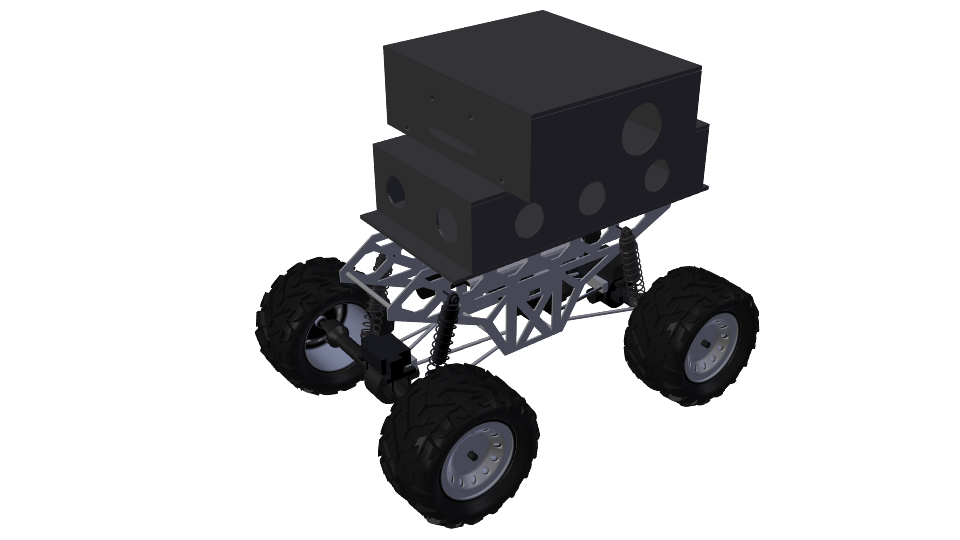
\includegraphics[width=10cm]{Chapters/Chapter2/Figures/base_diag.png}
		\caption{3D μοντέλο του συναρμολογημένου σασί της ρομποτικής πλατφόρμας Monstertruck.}
		\label{fig:chassis}
	\end{center}
\end{figure}

\bigskip
\subsection{Ηλεκτρονικός Εξοπλισμός}
% σύστηματα τροφοδοσίας, υπολογιστής, αισθήτηρες, κινητήρες, σερβοκινητήρες και ελεγκτές

\bigskip
\subsubsection{Υπολογιστής}
Το πιο σημαντικό τμήμα μία ρομποτικής πλατφόρμας και ιδιαίτερα μίας αυτόνομης ρομποτικής πλατφόρμας αποτελεί ο εγκέφαλος του, δηλαδή, το υπολογιστικό του σύστημα, που του επιτρέπει να ελέγχει τα υποσυστήματα του και να εκτελεί διεργασίες και αλγορίθμους. Η επιλογή του υπολογιστικού συστήματος, που εν τέλει, εγκαταστάθηκε στην ρομποτική πλατφόρμα \textit{Monstertruck}, βασίστηκε σε δύο κριτήρια. Πρώτο και βασικότερο κριτήριο επιλογής, αποτέλεσε η υπολογιστική ισχύς και κατά πόσο θα μπορούσε να εκτελεί τους απαιτούμενους αλγορίθμους ταυτόχρονα, αποδοτικά και χωρίς καθυστερήσεις. Το δεύτερο κριτήριο επιλογής, που λήφθηκε υπόψιν, ήταν, η κατανάλωση ισχύος, όσον αφορά τον χρόνο αυτονομίας.

\bigskip
Με βάση τα παραπάνω κριτήρια, τα υπολογιστικά συστήματα που εξετάστηκαν είναι το \textit{Raspberry Pi 2}, του \textit{Raspberry Pi Foundation} και το \textit{Odroid-XU4}, της \textit{Hardkernel}. Και οι δύο υπολογιστές, αυτοί, αποτελούν πλήρεις υπολογιστές, με Κεντρική Μονάδα Επεξεργασίας (CPU), μνήμη RAM, κάρτα γραφικών κλπ., σε εξαιρετικά μικρό μέγεθος και χαμηλές κατανάλωση ισχύος.

\begin{figure}[!ht]
	\begin{minipage}[t]{.49\textwidth}
 		\centering
		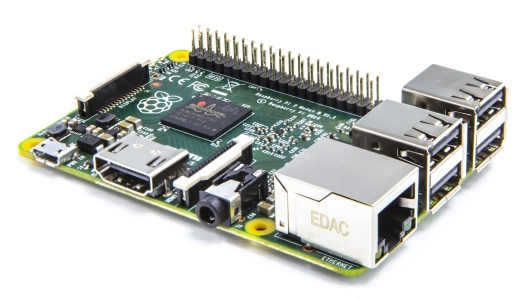
\includegraphics[width=0.6\linewidth]{Chapters/Chapter2/Figures/rpi2.jpg}
		\captionof{figure}{Raspberry Pi 2}
		\label{fig:rpi2}
	\end{minipage}
	\begin{minipage}[t]{.5\textwidth}		
		\centering
		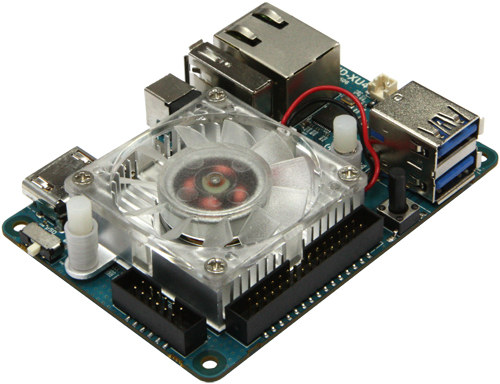
\includegraphics[width=0.5\linewidth]{Chapters/Chapter2/Figures/odroid-xu4.jpg}
		\captionof{figure}{Odroid-XU4}
		\label{fig:odroid-xu4}
	\end{minipage}
\end{figure}

\begin{table}[!ht]
	\caption{Προδιαγραφές Raspberry Pi 2 και Odroid-XU4.}
	\label{tab:computer_specs}
	\begin{center}
		\begin{tabular}{| l | c | c |}
	   		\hline
		   \textbf{Προδιαγραφές} & \textbf{Raspberry Pi 2} & \textbf{Odroid-XU4} \\ \hline
		   	CPU & Broadcom BCM2836 Arm7 & Samsung Exynos5422 ARM® \\ &Quad Core 900MHz Processor & Cortex™-A15 Quad 2.0GHz/\\ & & Cortex™-A7 Quad 1.4GHz\\ \hline
			GPU & Dual Core VideoCore IV® & Mali™-T628 MP6 OpenGL ES 3.0\\
			& Multimedia Co-Processor & / 2.0 / 1.1 and OpenCL 1.1 Full profile\\ 
			&  Open GL ES 2.0 &\\ \hline		   
		   RAM & 1GB LPDDR2 & 2GB LPDDR3 \\ \hline
		   USB 2.0 & 4 & 1\\ \hline
		   USB 3.0 & - & 2\\ \hline
		   Display & HDMI & HDMI\\ \hline
		   Sound & 4 pole Stereo output & HDMI Digital audio output\\ \hline
		   Storage & Micro SD & Micro SD ή eMMC 5.0\\ \hline
		   Ethernet & 10/100 & 10/100/1000\\ \hline
		  	Wifi & USB IEEE 802.11b/g/n & USB IEEE 802.11b/g/n 1T1R WLAN\\ \hline
		  	Περιφερειακά & 40-pin GPIO, UART, SPI, I2C & UART, 30-pin GPIO/IRQ/SPI/ADC\\
		  	& & 12-pin GPIO/I2S/I2C \\ \hline
		  	Power & 5V, 2A & 5V, 4A\\ \hline
		   Dimensions & $85 \times 56 \times 17 mm$ & $82 \times 58 \times 22 mm$\\\hline
	   \end{tabular}
	\end{center}
\end{table}

Αρχικά, χρησιμοποιήθηκε στην ρομποτική πλατφόρμα \textit{Monstertruck}, ο υπολογιστής \textit{Raspberry Pi 2}, αλλά, μετά από πειράματα και δοκιμές, με τους απαιτούμενους αλγορίθμους, για την λειτουργία του οχήματος, ως αυτόνομο ρομποτικό πράκτορα, διαπιστώθηκε, ότι, ο υπολογιστής \textit{Raspberry Pi 2},  είναι ανεπαρκής για την συγκεκριμένη εφαρμογή, για την οποία προορίζεται η ρομποτική πλατφόρμα. Σαν αποτέλεσμα, στην ρομποτική πλατφόρμα, τελικά χρησιμοποιήθηκε ο υπολογιστής \textit{Odroid-XU4}, που μετά από αντίστοιχα πειράματα, η απόδοση του κρίθηκε πλήρως ικανοποιητική.

\bigskip
\subsubsection{Αισθητήρες}
Μία εξαιρετικά σημαντική ιδιότητα, κάθε αυτόνομου ρομποτικού συστήματος, αποτελεί η αντίληψη του, όσον αφορά το περιβάλλον του. Συγκεκριμένα, η ρομποτική αντίληψη στηρίζεται σε ένα σύνολο αισθητήρων, που επιτρέπουν στο ρομποτικό σύστημα να λαμβάνει πληροφορίες σχετικά με το περιβάλλον του, σε μορφή κατανοητή και να αξιοποιήσιμη, από αυτό.

\bigskip
Οι ρομποτικοί αισθητήρες, χωρίζονται σε κατηγορίες, ανάλογα με την πηγή της πληροφορίας, σε \textit{ιδιοδεκτικούς (proprioceptive)} ή \textit{εξωδεκτικούς (exteroceptive)} \cite{autonomous_mobile_robots}, εάν η πληροφορία προέρχεται από το ίδιο το ρομποτικό σύστημα, ή από το περιβάλλον του, αντίστοιχα. Παραδείγματα \textit{ιδιοδεκτικών} αισθητήρων, αποτελούν, οι \textit{αισθητήρες μέτρησης θέσης, ταχύτητας και ροπής των κινητήρων}, \textit{γυροσκόπια}, \textit{αισθητήρες μέτρησης της φόρτισης των μπαταριών} κα. Αντίστοιχα, \textit{εξωδεκτικοί} αισθητήρες, θεωρούνται, οι \textit{αισθητήρες επαφής (tactile sensors)}, οι \textit{ηλεκτρονικές πυξίδες (compass, IMU)}, \textit{αισθητήρεςGPS}, οι \textit{υπέρυθροι, υπερηχητικοί και λέιζερ αισθητήρες απόστασης (range sensors)}, όπως επίσης και οι \textit{κάμερες}. Επίσης, χωρίζονται και με βάση την πηγή εκπομπής της πληροφορίας \cite{autonomous_mobile_robots} σε \textit{παθητικούς (passive)}, εάν μετρούν κάποια μορφή ενέργειας που προέρχεται από το περιβάλλον και σε \textit{ενεργητικούς (active)}, εάν εκπέμπουν ενέργεια στο περιβάλλον και έπειτα, μετρούν την αντίδραση του περιβάλλοντος. Με βάση, τον συγκεκριμένο ορισμό, \textit{αισθητήρες αφής}, \textit{ηλεκτρονικές πυξίδες} και \textit{κάμερες}, αποτελούν \textit{παθητικούς} αισθητήρες, ενώ \textit{κωδικοποιητές(encoders) κινητήρων}, \textit{GPS}, \textit{αισθητήρες απόστασης}, αποτελούν \textit{ενεργητικούς} αισθητήρες. 

\bigskip
Ένα αυτόνομο ρομποτικό όχημα, είναι προφανές, ότι απαιτεί αισθητήρες, από όλες τις παραπάνω κατηγορίες για να μπορεί να αντιληφθεί και να κινηθεί μέσα στο περιβάλλον του, αλλά και να αντιδράσει μ' αυτό. Ακολούθως, παρουσιάζεται το σύνολο των αισθητήρων, που περιλαμβάνει η ρομποτική πλατφόρμα \textit{Monstertruck}.

\bigskip
\begin{enumerate}
% Laser Scanner
\item
Οι πιο σημαντικοί αισθητήρες για ένα αυτόνομο ρομποτικό όχημα, είναι οι \textit{αισθητήρες απόστασης (range sensors)}, οι οποίοι, του προσφέρουν πληροφορία, σχετικά με την απόσταση του οχήματος από εμπόδια, επιτρέποντας του, με αυτόν τον τρόπο, μέσω κατάλληλων αλγορίθμων, να χαρτογραφεί τον περιβάλλοντα χώρο του, να ξέρει, ανά πάσα στιγμή, τη θέση του και να πλοηγείται, αυτόνομα, μέσα σε αυτόν, αποφεύγοντας συγκρούσεις.

Αντίστοιχα, στην ρομποτική πλατφόρμα \textit{Monstertruck}, για τους παραπάνω λόγους, εγκαταστάθηκε ένας \textit{Σαρωτής Λέιζερ (Laser Scanner) Hokuyo URG-04LX}. Ο αισθητήρας αυτός περιλαμβάνει μία περιστρεφόμενη κεφαλή \textit{μέτρησης απόστασης, μέσω ανίχνευσης φωτός (Light Detection and Ranging - LIDAR)}, περιμετρικά του αισθητήρα, σε εύρος $240^{\circ}$ και εμβέλεια $4m$.

\begin{figure}[!ht]
	\begin{minipage}[t]{.49\textwidth}
 		\centering
		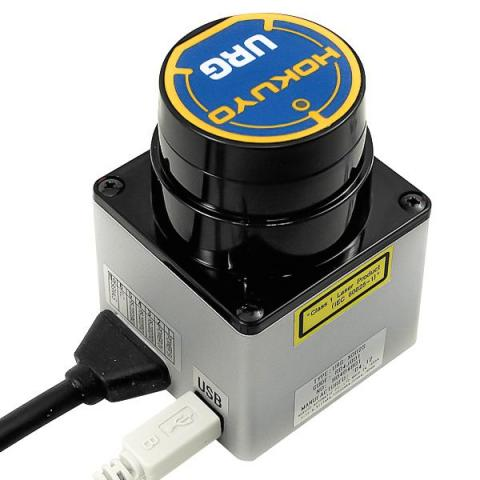
\includegraphics[width=0.6\linewidth]{Chapters/Chapter2/Figures/hokuyo.jpg}
		\captionof{figure}{Hokuyo URG-04LX.}
		\label{fig:hokuyo}
	\end{minipage}
	\begin{minipage}[t]{.49\textwidth}		
		\centering
 		\centering
		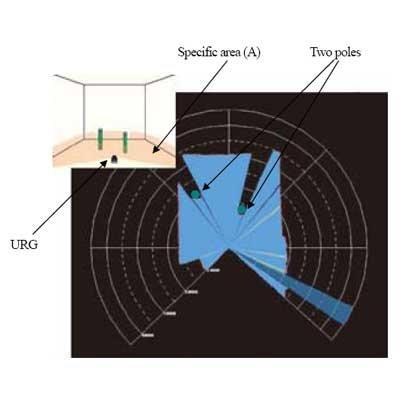
\includegraphics[width=0.75\linewidth]{Chapters/Chapter2/Figures/hokuyo_rays.jpg}
		\captionof{figure}{Ο Σαρωτής Λέιζερ Hokuyo URG-04LX σε δράση.}
		\label{fig:hokuyo_rays}
	\end{minipage}
\end{figure}

\bigskip

\begin{table}[!ht]
	\centering
	\captionof{table}{Προδιαγραφές Hokuyo URG-04LX}
	\label{tab:hokuyo_specs}
	\begin{tabular}{| l | c |}
		\hline
	   \textbf{Προδιαγραφές} & \textbf{Hokuyo URG-04LX} \\ \hline
	   Τροφοδοσία & 5VDC, 500mA\\ \hline
	   Εμβέλεια & 60 - 4\,095 mm \\ \hline
	   Περιοχή Μέτρησης & $240^{\circ}$\\ \hline
	   Ακρίβεια & $60 - 1000mm: \pm 10$ \\
   		& $1000 - 4095mm: 1\%$ \\ \hline
	  	Γωνιακή Ακρίβεια & $0.36^{\circ} (360^{\circ}/1024)$ \\ \hline
	  	Διεπαφή & USB, RS232 \\ \hline
	  	Διαστάσεις & $50 \times 50 \times 70 mm$ \\ \hline
	\end{tabular}
\end{table}

% IMU
\bigskip
\item
Ένα, άλλο είδος αισθητήρων, ιδιαίτερα δημοφιλές και απαραίτητο στις περισσότερες ρομποτικές εφαρμογές, αποτελούν οι \textit{αισθητήρες κατεύθυνσης (heading sensors)} \cite{autonomous_mobile_robots}. Στην κατηγορία, αυτή, ανήκουν τα \textit{γυροσκόπια (gyroscopes)}, τα \textit{κλινόμετρα (inclinometers)} και οι \textit{πυξίδες (compasses)}. Οι αισθητήρες, αυτοί, χρησιμοποιούνται για να καθοριστούν ο \textit{προσανατολισμός (orientation / yaw)} και η \textit{κλίση (pitch, roll)} του ρομποτικού οχήματος, αλλά και σε συνδυασμό με μετρήσεις ταχύτητας για την εκτίμηση της θέσης του (\textit{dead reckoning}).

Η ρομποτική πλατφόρμα \textit{Monstertruck} χρησιμοποιεί την \textit{πυξίδα Compass OS4000}, της \textit{Ocean Server}. Ο αισθητήρας αυτός, συνδυάζει ένα \textit{μαγνητόμετρο (magnetometer)}, τριών αξόνων και ένα \textit{επιταχυνσιόμετρο (accelerometer)}, τριών αξόνων. Το μαγνητόμετρο χρησιμοποιεί το μαγνητικό πεδίο της γης, για να μετρήσει τον απόλυτο προσανατολισμό, ως προς τους τρεις άξονες $x, y, z$, ενώ το επιταχυνσιόμετρο, μετράει μεταβολές στην ταχύτητα, ως προς τους τρεις άξονες $x, y, z$.

\begin{figure}[!ht]
	\begin{minipage}[b]{0.45\textwidth}
		\centering
		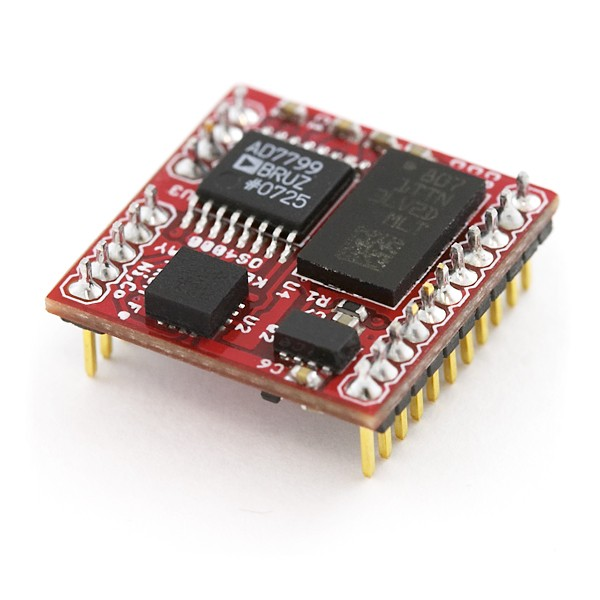
\includegraphics[width=0.5\linewidth]{Chapters/Chapter2/Figures/compassOS4000.jpg}
		\captionof{figure}{Compass OS4000.}
		\label{fig:compassOS4000}
	\end{minipage}		
	\begin{minipage}[b]{0.54\textwidth}
		\centering
		\begin{tabular}{| l | c |}
			\hline
			\textbf{Προδιαγραφές} & \textbf{Compass OS4000}\\ \hline
			Τροφοδοσία & $3.3-5VDC, 30mA @ 3.3V$\\ \hline
			Σειριακή Διεπαφή& TTL 4800-115000 baud\\
			Επικοινωνίας  & 8 bit, 1 stop, no parity\\ \hline
			Συχνότητα & $0.01-40Hz$\\ \hline
			Ακρίβεια Αζιμούθιου & $<0.5^{\circ}, 0.1^{\circ}$ resolution\\ \hline
			Ακρίβεια Κλίσης & $<0.5^{\circ}, 0.1^{\circ}$ resolution\\ \hline
			Διαστάσεις & $15 \times 15 mm$\\ \hline
		\end{tabular}
		\captionof{table}{Προδιαγραφές Compass OS4000}
		\label{tab:compassOS4000}
	\end{minipage}
\end{figure}

Η \textit{πυξίδα Compass OS4000}, για την ώρα, χρησιμεύει, μόνο, για την, εύρεση της κλίσης (pitch, roll) του ρομπότ, έτσι ώστε να σταθεροποιείται στο οριζόντιο επίπεδο ο \textit{σαρωτής λέιζερ}, που αναφέρθηκε παραπάνω, μέσω ενός μηχανισμού \textit{σταθεροποιητή pitch-roll}, που αποτελείται από δύο. \textit{σερβοκινητήρες}. Παρόλα αυτά, η \textit{πυξίδα}, μπορεί να χρησιμοποιηθεί, κάλλιστα και για την \textit{εκτίμηση κατάστασης (θέση και προσανατολισμός)} του οχήματος, για την επέκταση \textit{αλγορίθμων ακολούθησης μονοπατιού}, με βάση την ομαλότητα του εδάφους, βάση της τρέχουσα κλίσης του οχήματος, αλλά και σε ρουτίνες ασφαλείας, σε περίπτωση επικίνδυνων επιπέδων κλίσης του οχήματος, που μπορεί να προκαλέσουν ανατροπή.

% Camera
\bigskip
\item
Η όραση αποτελεί την πιο ισχυρή αίσθηση του ανθρώπου. Προσφέρει ένα τεράστιο όγκο πληροφορίας για το περιβάλλον και διευκολύνει την διάδραση του με αυτό. Στα ρομποτικά συστήματα, η αίσθηση της όραση προσεγγίζεται με \textit{κάμερες}, οι οποίες καταγράφουν την ίδια πληροφορία, σε μεγάλο βαθμό που συγκεντρώνει και το ανθρώπινο μάτι.

Στα ρομποτικά συστήματα, \textit{κάμερες}, μπορεί να χρησιμοποιούνται για επίβλεψη και χειρισμό ρομποτικών συστημάτων, αλλά μεγαλύτερο ενδιαφέρον, παρουσιάζει ο κλάδος της \textit{ρομποτικής όρασης}, που ασχολείται με την δημιουργία αλγορίθμων, που εξάγουν πληροφορία, από τις εικόνες, που παράγει μία \textit{κάμερας}. Για παράδειγμα, \textit{κάμερες} και αλγόριθμοι \textit{ρομποτικής όρασης}, χρησιμοποιούνται για αναγνώριση αντικειμένων, προσώπων και προτύπων, γενικότερα, αλλά, ακόμα και \textit{χαρτογράφηση περιβάλλοντος} και \textit{εκτίμηση κατάστασης (Visual SLAM, Monocular SLAM)} κα.

Στην ρομποτική πλατφόρμα \textit{Monstertruck}, είναι εγκατεστημένη, μία απλή \textit{web κάμερα Logitech Portable Webcam C905}, η οποία, χρησιμοποιήθηκε, στα πλαίσια της παρούσας εργασίας, μονάχα για επίβλεψη κατά τον χειρισμό, ή την αυτόνομη λειτουργία της ρομποτικής πλατφόρμας. Παρόλα αυτά, όπως αναφέρθηκε παραπάνω, με την εκμετάλλευση της πληροφορίας από την κάμερα, μέσω κατάλληλων αλγορίθμων, η λειτουργικότητα της ρομποτικής πλατφόρμας, μπορεί να εξελιχθεί σημαντικά.

\begin{figure}[!ht]
	\centering
	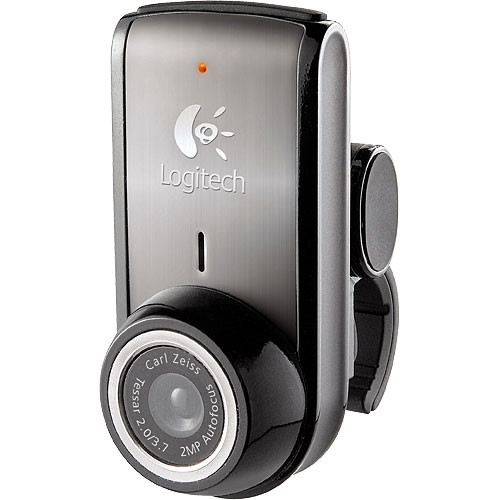
\includegraphics[width=.4\linewidth]{Chapters/Chapter2/Figures/webcam.jpg}
	\caption{Logitech Portable Webcam C905.}
	\label{fig:webcam}
\end{figure}


% motor encoders, hall sensors
\bigskip
\item
Σε ρομποτικά συστήματα, με κινούμενα μέρη, όπως είναι προφανές, χρησιμοποιούνται κινητήρες και σερβοκινητήρες. Για τον ακριβή έλεγχο και παρακολούθηση, αυτών, είναι απαραίτητη η ύπαρξη αισθητήρων, που προσφέρουν πληροφορία, σχετικά με την θέση, ταχύτητα, επιτάχυνση, φορτίο, ρεύμα, τροφοδοσία ή θερμοκρασία, κατά την λειτουργία τους. Στη ρομποτική πλατφόρμα \textit{Monstertruck}, χρησιμοποιείται, ένας \textit{αισθητήρες Hall}, για τον κινητήρα των τροχών και \textit{κωδικοποιητές (encoders)}, για τον κινητήρα και τους σερβοκινητήρες του οχήματος. 

Ο \textit{αισθητήρας Hall}, είναι ένας μετατροπέας, που μεταβάλλει την τάση εξόδου του, ως αντίδραση στις μεταβολλές ενός μαγνητικού πεδίου. Στους κινητήρες χρησιμοποιείται ως μετρητής των στροφές ανά λεπτό. Είναι οικονομικός αισθητήρας, μπορεί να δουλέψει σε υψηλές συχνότητες και δεν επηρεάζεται από φαινόμενα θορύβου μηχανικών επαφών (contact bounce), αλλά, έχει μικρή ακρίβεια και είναι επιρρεπείς σε σημαντικές αποκλίσεις (drift).

Οι \textit{κωδικοποιητές}, είναι μία κατηγορία αισθητήρων που χρησιμοποιούνται, για την μέτρηση της θέσης, σε απλές περιπτώσεις, ή ταχύτητας του άξονα ενός κινητήρα. Η μέτρηση αυτή χρησιμοποιείται από το κύκλωμα κλειστού βρόχου, ενός κινητήρα για έλεγχο θέσης ή ταχύτητας. Οι απλοί, \textit{συμβατικοί σερβοκινητήρες (hobby servos)}, του εμπορίου, χρησιμοποιούν \textit{περιστροφικούς κωδικοποιητές} στην μορφή ποτενσιομέτρων (\textit{rotary / shaft encoders}), που μεταβάλλουν την τάση εξόδου τους, ανάλογα με την θέση του άξονα του σερβοκινητήρα. Αντίθετα, οι \textit{βιομηχανικοί κινητήρες}, συνήθως χρησιμοποιούν \textit{οπτικούς κωδικοποιητές (optical encoders)}, οι οποίοι, αποτελούνται από έναν δίσκο με διαφανείς και αδιαφανείς περιοχές και και ζεύγη φωτοεκπομπών και φωτοδεκτών, που διαβάζει τα μοτίβα του δίσκου και συμπεραίνει την θέση του άξονα του κινητήρα.

\bigskip
\begin{figure}[!ht]
	\centering
	\subfloat[Φαινόμενο Hall Κινητήρα.]{
		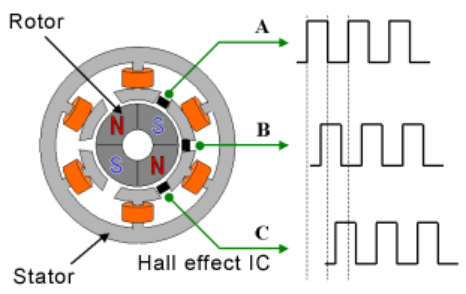
\includegraphics[width=0.4\linewidth]{Chapters/Chapter2/Figures/motor_hall_effect.png}
		\label{fig:hall_sensor}}
	\subfloat[Περιστροφικός Κωδικοποιητής.]{
		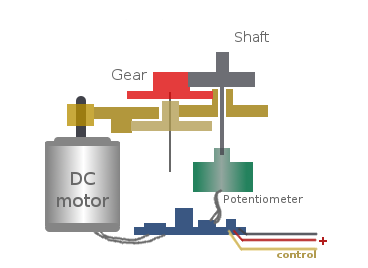
\includegraphics[width=0.4\linewidth]{Chapters/Chapter2/Figures/servo_internals.png}
		\label{fig:rotary_encoder}}\\
	\subfloat[Οπτικός Κωδικοποιητής.]{
		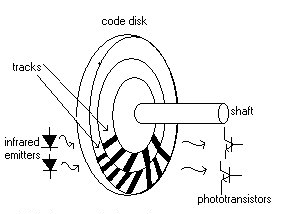
\includegraphics[width=0.4\linewidth]{Chapters/Chapter2/Figures/optical_encoder.png}
		\label{fig:optical_encoder}}
	\caption{Αισθητήρες θέσης και ταχύτητας κινητήρων.}
\end{figure}


% battery monitor
\bigskip
\item
Η ρομποτική πλατφόρμα \textit{Monstertruck}, τροφοδοτείται, μέσω, επαναφορτιζόμενων μπαταριών \textit{Λιθίου - Πολυμερών (LiPo)}, που συνδυάζουν υψηλή χωρητικότητα, μικρό όγκο και βάρος, σε σύγκριση με άλλους τύπους μπαταριών. Ένα σημαντικό πρόβλημα των μπαταριών \textit{LiPo}, είναι η ασφάλεια τους, καθώς σε περίπτωση υπερφόρτισης, αποφόρτισης, βραχυκυκλώματος, κρούσης ή διείσδυσης, μπορεί να προκληθεί καταστροφική ζημιά, όπως ρήξη συσκευασίας, διαρροή ηλεκτρολύτη και φωτιά. Επίσης, κακή χρήση της μπαταρίας, μέσω υπερφορτίσεων και αποφορτίσεων πέρα από τα επιτρεπτά επίπεδα, προκαλεί μείωση της χωρητικότητας και του χρόνου ζωής της μπαταρίας. Καθίσταται, επομένως, απαραίτητη, η χρήση ενός αισθητήρα, που θα μετρά τα επίπεδα τάσης της μπαταρίας και θα τα μεταδίδει στον κεντρικό υπολογιστή του ρομποτικού συστήματος, στον οποίο θα λειτουργεί μία διεργασία, που θα λαμβάνει την πληροφορία αυτή, θα την επεξεργάζεται κατάλληλα (πχ. φιλτράρισμα θορύβου) και θα εξάγει συμπεράσματα και θα ειδοποιεί τον επιβλέπον / χειριστή, σε περίπτωση που η μπαταρία χρειάζεται φόρτιση ή σε περίπτωση που παρεκκλίνει από τα επιτρεπτά όρια.

Για την μέτρηση της τάσης της μπαταρίας, απαιτείται ένας αισθητήρας που θα μετατρέπει την αναλογική τάση σε ψηφιακή πληροφορία. Τον σκοπό αυτό εξυπηρετούν οι \textit{Μετατροπείς Αναλογικού Σήματος σε Ψηφιακό (ADC)}, οι οποίοι μετατρέπουν μία αναλογική τάση σε έναν ψηφιακό αριθμό. Η διαδικασία της μετατροπής, περιλαμβάνει κβαντισμό και περιοδική δειγματοληψία, της τάσης εισόδου και σαν αποτέλεσμα εισάγει ένα μικρό σφάλμα μετατροπής, το οποίο στην προκειμένη περίπτωση, δεν επηρεάζει, σημαντικά, την εφαρμογή. Οι αισθητήρες \textit{ADC}, περιγράφονται, συνήθως, από μία μέγιστη τάση εισόδου (πχ. $5V$). Επειδή, όμως στην ρομποτική πλατφόρμα χρησιμοποιούνται μπαταρίες LiPo, με ονομαστική τάση $22.2V$ (μέγιστη τάση $25.2V$), απαιτείται μία κλιμάκωση της τάσης εισόδου. Για τον λόγο αυτό, η τάση εισόδου του μετατροπέα ADC, κλιμακώνεται, μέσω ενός διαιρέτη τάσης, με σχέση 1:10, από 0-25.2V σε 0-2.52V. Επίσης, λόγω των μεγάλων διαταραχών, στην τάση της μπαταρίας, κατά την λειτουργία της ρομποτικής πλατφόρμας, χρησιμοποιήθηκε ένα \textit{χαμηλοπερατό φίλτρο RC}. 

\begin{figure}[!ht]
	\centering
	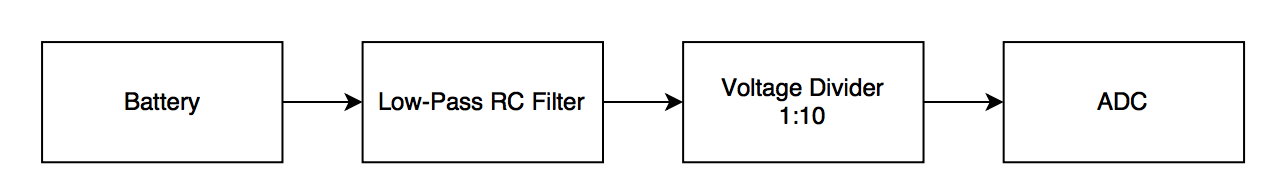
\includegraphics[width=\linewidth]{Chapters/Chapter2/Figures/rc_filter_divider.png}
	\caption{Στάδια επεξεργασίας τάσης μπαταρίας για μέτρηση της σε ADC.}
	\label{fig:rc_filter_divider}
\end{figure}

\end{enumerate}


\bigskip
\subsubsection{Κινητήρας}
Το τηλεκατευθυνόμενο όχημα GroundPounder, αρχικά, περιελάμβανε έναν \textit{Brushed DC ηλεκτρικό κινητήρα}, με μέγιστη ταχύτητα, περίπου, $30\,000rpm$, ο οποίος ελεγχόταν από έναν ελεγκτή \textit{ESC}, με δυνατότητες ελέγχου ταχύτητας και φοράς. Παρόλα αυτά, λόγω της μικρής ακρίβειας, ελέγχου ταχύτητας και την απουσία \textit{κωδικοποιητή} ή άλλων αισθητήρων για την παροχή μετρήσεων, σχετικά την πραγματική ταχύτητα του κινητήρα, κάθε στιγμή, σε συνδυασμό, με τις υψηλές απαιτήσεις ακριβείας των ρομποτικών εφαρμογών, κρίθηκε σκόπιμο, το εν λόγω σύστημα κινητήρα και ελεγκτή, να αντικατασταθεί.

\begin{figure}[!ht]
	\begin{minipage}{.49\textwidth}
 	\centering
		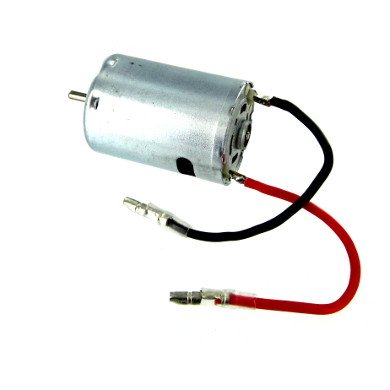
\includegraphics[width=0.6\linewidth]{Chapters/Chapter2/Figures/original_motor.jpg}
		\captionof{figure}{
			Ο κινητήρας Brushed 540 του τηλεκατευθυνόμενου οχήματος GroundPounder.}
		\label{fig:original_motor}
	\end{minipage}
	\begin{minipage}{.5\textwidth}		
		\centering
		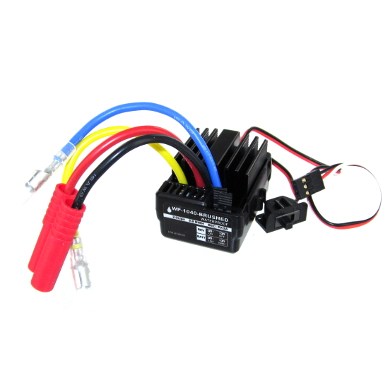
\includegraphics[width=0.6\linewidth]{Chapters/Chapter2/Figures/esc.jpg}
		\captionof{figure}{
			Ο ελεγκτής ESC B7003SR του τηλεκατευθυνόμενου οχήματος GroundPounder.}
		\label{fig:esc}
	\end{minipage}
\end{figure}

\bigskip
Για την αντικατάσταση, λοιπόν του παραπάνω συστήματος κινητήρα και ελεγκτή, επιλέχθηκαν, από τον διαθέσιμο εξοπλισμό της ομάδας \textit{P.A.N.D.O.R.A}, ένας κινητήρας, με αντίστοιχο ελεγκτή, της εταιρείας \textit{maxon motor}. Ο κινητήρας <TODO: τύπος>, είναι ένας \textit{Brushless EC κινητήρας}, με μέγιστη ταχύτητα $18000rpm$, με \textit{ψηφιακό κωδικοποιητή (encoder)}, για μέτρηση της θέσης του άξονα του κινητήρα, όπως επίσης και \textit{αισθητήρα Hall} για μέτρηση των στροφών του κινητήρα, ανά λεπτό. Επίσης, περιλαμβάνει \textit{κιβώτιο ταχυτήτων(gearbox)}, με σχέση 1:66. Αντίστοιχα, ως ελεγκτής, επιλέχθηκε ο \textit{EPOS 24/1}, της \textit{maxon motor}. Ο ελεγκτής αυτός, αποτελεί ένα μικρού μεγέθους, ψηφιακό, έξυπνο ελεγκτή, με δυνατότητες ελέγχου 
θέσης, ταχύτητας και ρεύματος.

\begin{figure}[!ht]
	\begin{minipage}{.49\textwidth}		
		\centering
		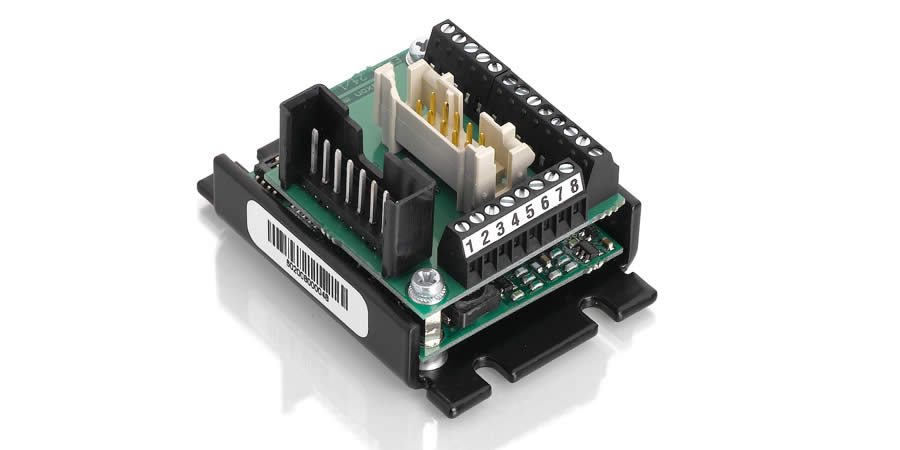
\includegraphics[width=0.8\linewidth]{Chapters/Chapter2/Figures/maxon_motor.jpg}
		\captionof{figure}{
			Ο κινητήρας maxon EC <TODO: τύπος και σωστή εικόνα>, της maxon motor.}
		\label{fig:maxon_motor}
	\end{minipage}
	\begin{minipage}{.5\textwidth}
 	\centering
		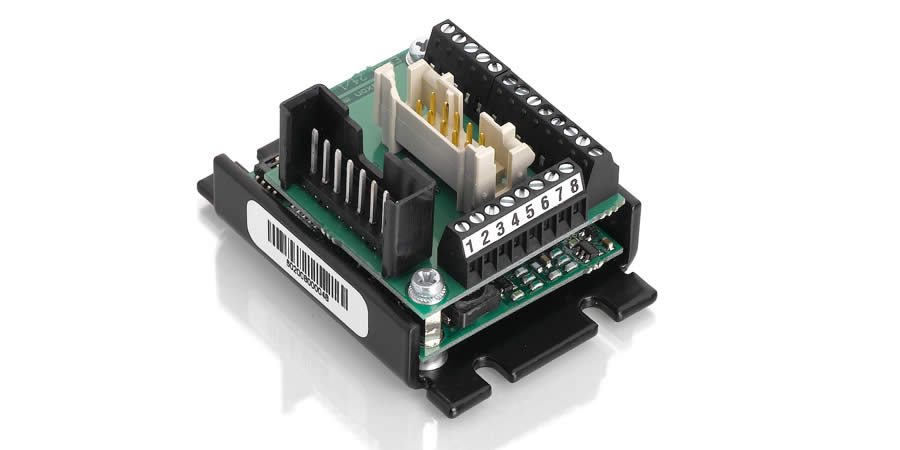
\includegraphics[width=0.8\linewidth]{Chapters/Chapter2/Figures/epos241.jpg}
		\captionof{figure}{
			Ο έξυπνος ελεγκτής κινητήρα, EPOS 24/1, της maxon motor \cite{epos241_manual}.}	
		\label{fig:epos241}
	\end{minipage}
\end{figure}

Ο κινητήρας \textit{<TODO: τύπος>}, συνδέεται με τον ελεγκτή \textit{EPOS 24/1}, μέσω δύο καλωδίων, ένα για τον έλεγχο του κινητήρα και για λήψη μετρήσεων από τον \textit{αισθητήρα Hall} και το άλλο, για λήψη μετρήσεων από τον \textit{ψηφιακό κωδικοποιητή}. Ο ελεγκτής \textit{EPOS 24/1}, επίσης, απαιτεί σύνδεση σε τροφοδοσία 9-24VDC, 1Α, ενώ παράλληλα, για επικονωνία με ηλεκτρονικό υπολογιστή, χρησιμοποιεί το πρωτόκολλο επικοινωνίας \textit{RS232}, χωρίς χειραψία, μέσω της ελάχιστης συνδεσμολογίας \textit{RS232} (RX, TX, Ground).

\begin{figure}[!ht]
		\centering
		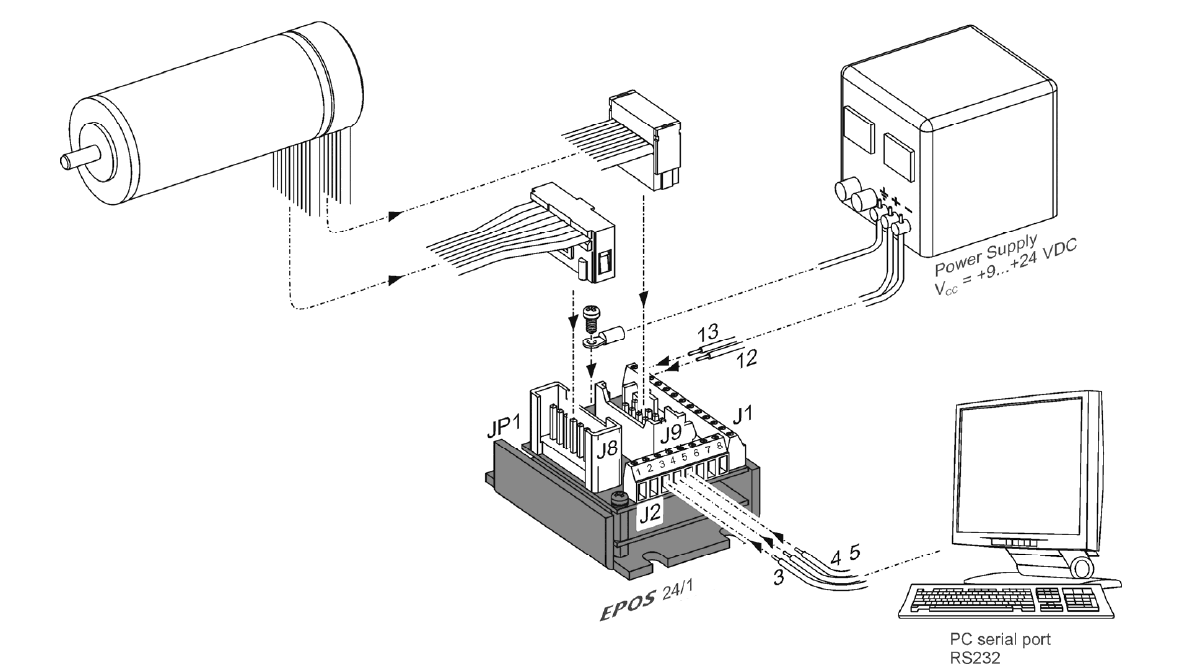
\includegraphics[width=0.7\linewidth]{Chapters/Chapter2/Figures/motor_minimum_wiring.png}
		\caption{Καλωδίωση Κινητήρα, Ελεγκτή και Υπολογιστή \cite{epos241_manual}.}
		\label{fig:motor_minimum_wiring}
\end{figure}

O ελεγκτής \textit{EPOS 24/1}, όπως προαναφέρθηκε, επιτρέπει την επικοινωνία με τον κεντρικό υπολογιστή της ρομποτικής πλατφόρμας, μέσω του πρωτοκόλλου διεπαφής \textit{RS232}. Παρόλα αυτά, ο κεντρικός υπολογιστής, δεν διαθέτει διεπαφή \textit{RS232} και επομένως, απαιτείται, ένας ενδιάμεσος κόμβος, ο οποίος θα καθιστά δυνατή την επικοινωνία μεταξύ τους. Το ρόλο αυτό, στην προκειμένη περίπτωση, εξυπηρετεί ένα \textit{μετατροπέας διεπαφής RS232 σε USB} (σχήμα \ref{fig:rs232_to_usb_adapter}).

\begin{figure}[!ht]
		\centering
		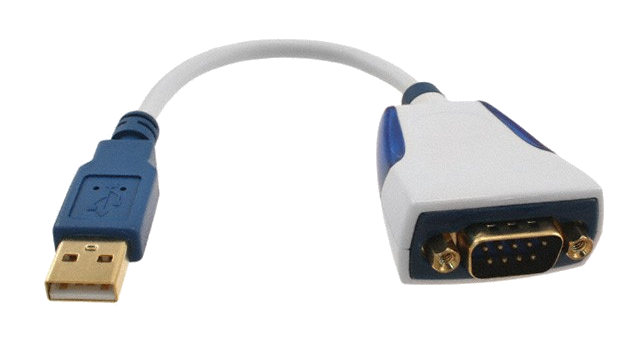
\includegraphics[width=.35\linewidth]{Chapters/Chapter2/Figures/rs232_to_usb_adapter.png}
		\caption{Μετατροπέας διεπαφής RS232 σε USB.}
		\label{fig:rs232_to_usb_adapter}
\end{figure}

\bigskip
\subsubsection{Σερβοκινητήρες}
Οι σερβοκινητήρες είναι κινητήρες, που επιτρέπουν ακριβή έλεγχο θέσης, ταχύτητας και επιτάχυνσης. Οι \textit{συμβατικοί σερβοκινητήρες} αποτελούνται από έναν DC κινητήρα, σε συνδυασμό με \textit{γρανάζια μετάδοσης}, έναν \textit{αισθητήρα θέσης}, συνήθως \textit{περιστροφικό κωδικοποιητή (rotary encoder)} και ένα κύκλωμα ελέγχου. Οι απλοί, συμβατικοί σερβοκινητήρες ελέγχονται, μέσω σημάτων Διαμόρφωσης Πλάτους Παλμού (PWM), αλλά υπάρχει, βέβαια και μία κατηγορία σερβοκινητήρων, οι λεγόμενοι \textit{έξυπνοι σερβοκινητήρες (smart servo motors)}, οι οποίοι έχουν ενσωματωμένο μικροελεγκτή. Ο μικροελεγτκής, αυτός, προσφέρει, υψηλότερη ακρίβεια ελέγχου, ευρωστία στο θόρυβο και αμφίδρομη επικοινωνία, μέσω σειριακού πρωτοκόλλου, συνήθως {TTL Full-Duplex} ή \textit{Half-Duplex} και \textit{RS485}. Τέλος, ένα σημαντικό πλεονέκτημα, των έξυπνων σερβοκινητήρων, έναντι των συμβατικών, είναι η παροχή πληροφορίας θέσης (position feedback), εξαιρετικής σημασίας για ρομποτικές εφαρμογές.

\bigskip
Στην ρομποτική πλατφόρμα \textit{Monstertruck} χρησιμοποιούνται συνολικά τέσσερις σερβοκινητήρες, δύο από τους οποίους είναι \textit{συμβατικοί} και οι άλλοι δύο, \textit{έξυπνοι}.

\bigskip
Οι δύο \textit{συμβατικοί σερβοκινητήρες}, χρησιμοποιούνται στο σύστημα \textit{τετραδιεύθυνσης} της ρομποτικής πλατφόρμας, που θα αναλυθεί στην αντίστοιχη ενότητα. Είναι τύπου \textit{Hitek HS-7954TH ??? <TODO>}, με ροπή $15kg/cm$ στα $6V$ και ανάλυση $<TODO: Resolution>$.

\bigskip
Ο έλεγχος των δύο σερβοκινητήρων πραγματοποιείται από έναν ελεγκτή \textit{Micro Maestro 6 - Channel USB Servo Controller}, της \textit{Pololu}. Ο ελεγκτής, αυτός, προσφέρει αποδοτικό έλεγχο σερβοκινητήρων, υψηλής ακρίβειας, με ενσωματωμένο έλεγχο ταχύτητας και επιτάχυνσης, έξι κανάλια ελέγχου και επικοινωνία, μέσω σειριακού πρωτοκόλλου \textit{USB}.

\begin{figure}[!ht]
	\begin{minipage}[t]{.49\textwidth}		
		\centering
		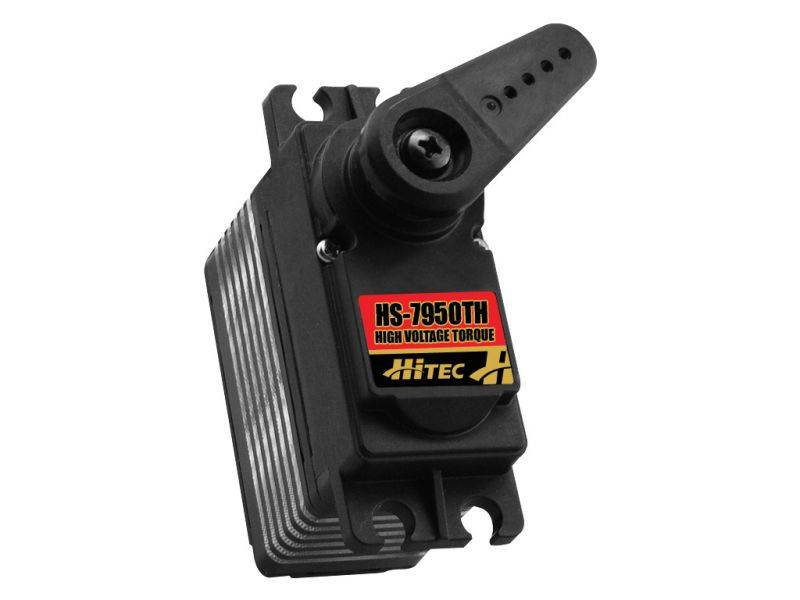
\includegraphics[width=0.5\linewidth]{Chapters/Chapter2/Figures/hitek_servo.jpg}
		\caption{Σερβοκινητήρας Hitek HS-7954TH.}
		\label{fig:hitek_servo}
	\end{minipage}
	\begin{minipage}[t]{.5\textwidth}
 	\centering
		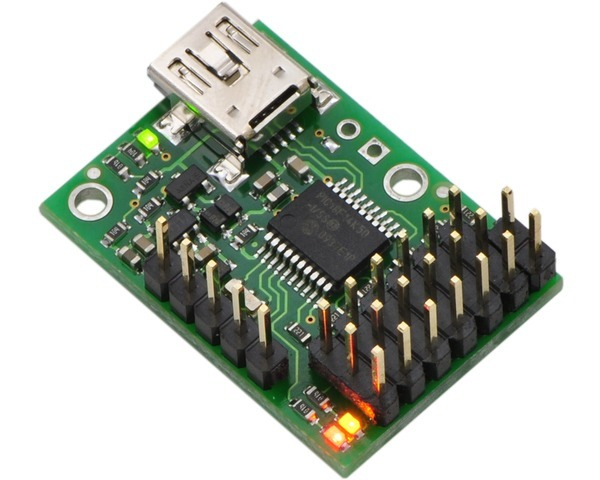
\includegraphics[width=0.5\linewidth]{Chapters/Chapter2/Figures/pololu_maestro.jpg}
		\captionof{figure}{Pololu Micro Maestro 6-Channel USB Servo Controller}
		\label{fig:pololu_maestro}
	\end{minipage}
\end{figure}

\begin{figure}[!ht]
		\centering
		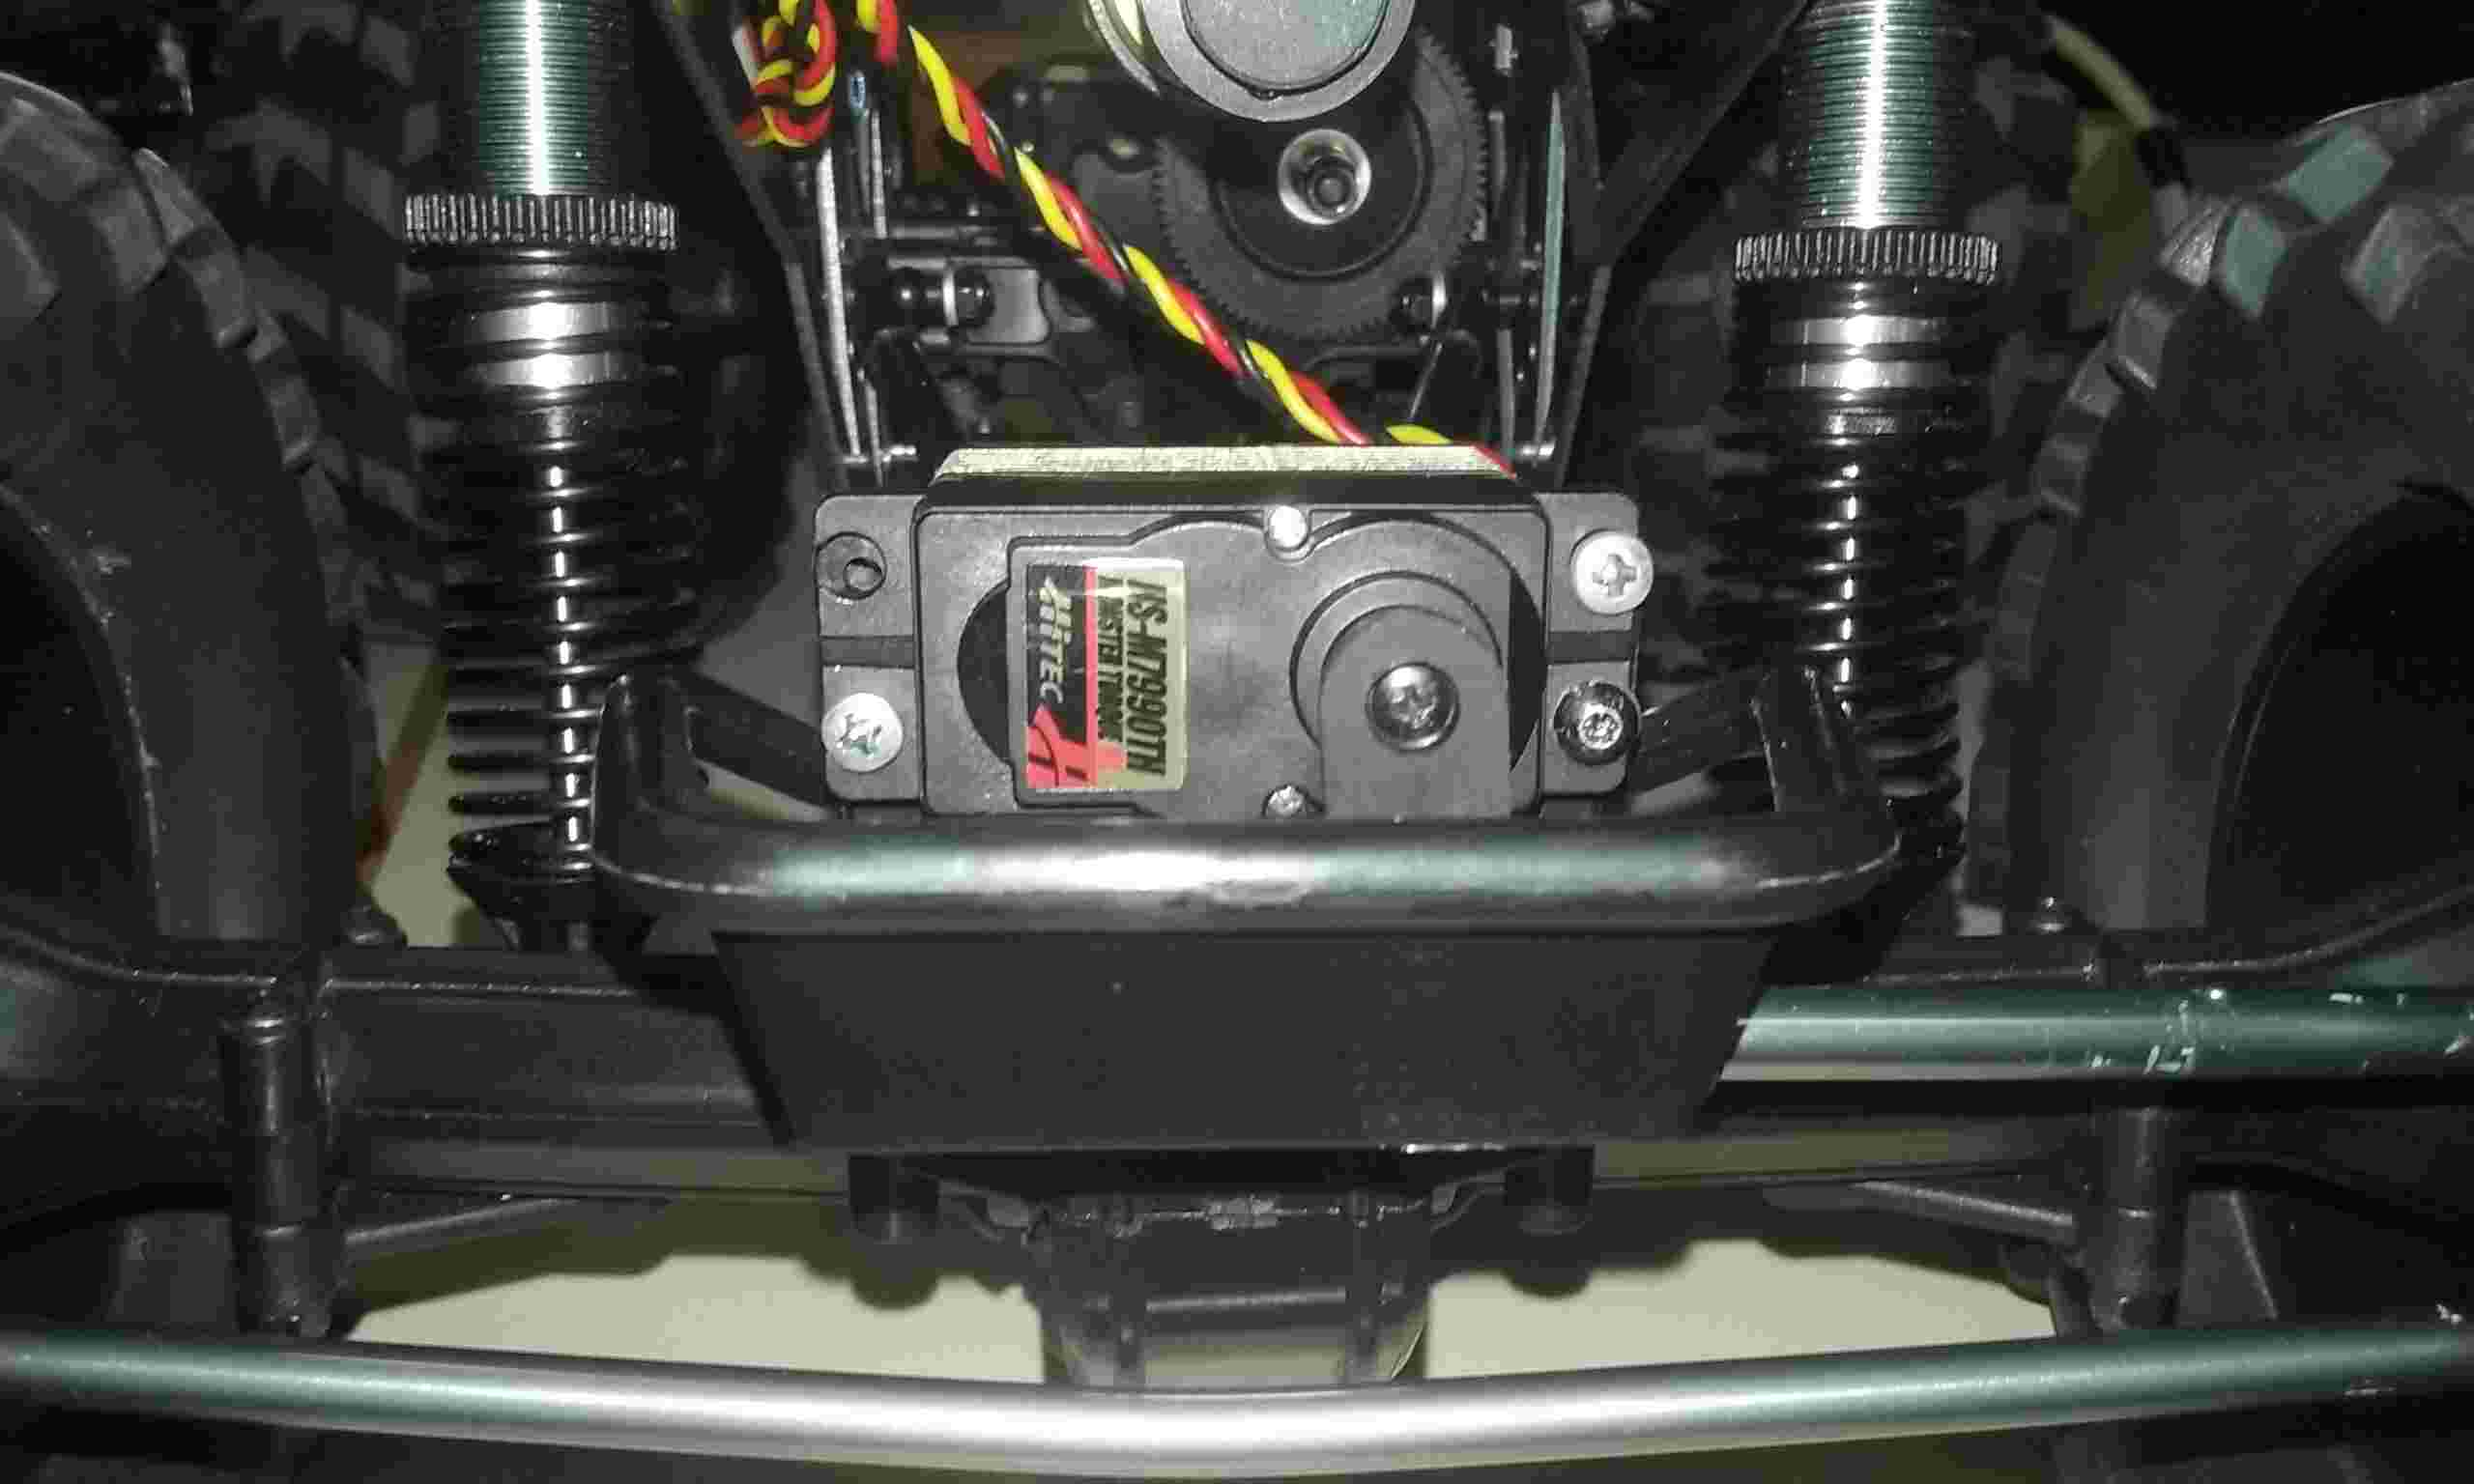
\includegraphics[width=0.5\linewidth]{Chapters/Chapter2/Figures/steering_servo.jpg}
		\caption{Σερβοκινητήρας στρέψης των τροχών.}
		\label{fig:servo_steering}
\end{figure}

\bigskip
Οι δύο \textit{έξυπνοι σερβοκινητήρες}, χρησιμοποιούνται ως \textit{μηχανισμός σταθεροποίησης (Pitch-Roll Stabilizer)} του \textit{Σαρωτή Λέιζερ}, που αναφέρθηκε παραπάνω, λαμβάνοντας υπόψιν πληροφορία για την κλίση του οχήματος, μέσω της πυξίδας \textit{Compass OS4000}. Ο μηχανισμός αυτός είναι απαραίτητος για την αξιόπιστη χαρτογράφηση χώρου με ανώμαλο έδαφος.

\bigskip
Οι \textit{έξυπνοι σερβοκινητήρες} του \textit{μηχανισμού σταθεροποίησης} του \textit{Σαρωτή Λέιζερ}, είναι τύπου \textit{Dynamixel AX-12A}, της \textit{Robotis}. Οι \textit{έξυπνοι σερβοκινητήρες Dynamixel AX-12}, έχουν την δυνατότητα, να παίρνουν μετρήσεις, σχετικά με την ταχύτητα, θέση, θερμοκρασία, τάση και φορτίο και να αντιδρούν ανάλογα με την περίπτωση και να μεταδίδουν αυτήν την πληροφορία, στον υπολογιστή του ρομποτικού συστήματος.

\begin{figure}[!ht]
	\begin{minipage}[b]{0.44\textwidth}
		\centering
		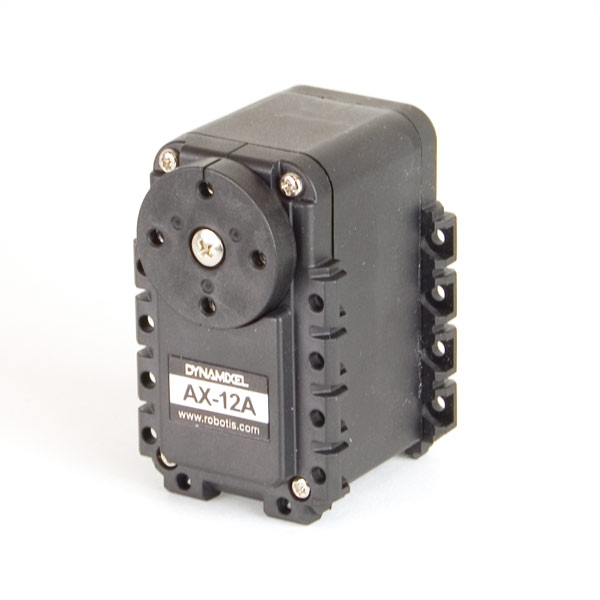
\includegraphics[width=0.8\linewidth]{Chapters/Chapter2/Figures/dxl_ax_12a.png}
		\caption{Σερβοκινητήρας Dynamixel\\ AX-12A, της Robotis.}
		\label{fig:dxl_ax_12a}
	\end{minipage}		
	\begin{minipage}[b]{0.55\textwidth}
		\centering
		\begin{tabular}{| l | c |}
			\hline
			\textbf{Προδιαγραφές} & \textbf{Dynamixel AX-12A}\\ \hline
			Τροφοδοσία & $9-12VDC, 900mA$\\ \hline
			Σειριακή Διεπαφή& 3-pin TTL Half-Duplex\\
			Επικοινωνίας  & 7343bps ~ 1Mbps\\ \hline
			Περιστροφή & $300^{\circ}$, ή συνεχής περιστροφή\\ \hline
			Μέγιστη Ροπή & $15.3 kg \cdot cm$\\ \hline
			Μέγιστη Ταχύτητα & 59 RPM \\ (χωρίς φορτίο) & 0.169sec/60°\\ \hline
			Feedback & Θέσης, Φορτίου,\\& Θερμοκρασίας, Τάσης\\ \hline
			Διαστάσεις & $32 \times 50 \times 40 mm$\\ \hline
		\end{tabular}
		\captionof{table}{Προδιαγραφές σερβοκινητήρα Dynamixel AX-12A, της Robotis}
		\label{tab:dxl_ax_12a_specs}
	\end{minipage}
\end{figure}


\bigskip
Η επικοινωνία, μεταξύ του υπολογιστή και των \textit{έξυπνων σερβοκινητήρων}, επιτυγχάνεται μέσω του \textit{αντάπτορα USB2Dynamixel}, ο οποίος επικοινωνεί με τον υπολογιστή, μέσω σειριακού πρωτοκόλλου \textit{USB} και με τους \textit{έξυπνους σερβοκινητήρες}, μέσω σειριακής επιικοινωνίας \textit{TTL}. Επίσης, οι δύο \textit{έξυπνοι σερβοκινητήρες}, συνδέονται, μεταξύ τους, σειριακά, μέσω τοπολογίας \textit{Daisy Chain}.

\begin{figure}[!ht]
	\begin{minipage}[t]{.49\textwidth}
 	\centering
		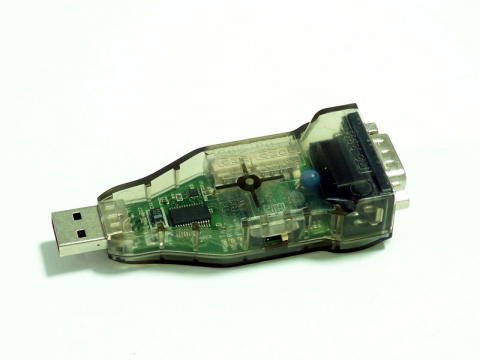
\includegraphics[width=0.7\linewidth]{Chapters/Chapter2/Figures/usb2dynamixel.png}
		\captionof{figure}{Αντάπτορας USB2Dynamixel,\\ της Robotis.}
		\label{fig:usb2dynamixel}
	\end{minipage}
	\begin{minipage}[t]{.5\textwidth}		
		\centering
		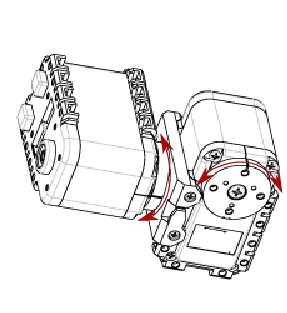
\includegraphics[width=0.6\linewidth]{Chapters/Chapter2/Figures/pitch_roll_dxl.png}
		\caption{Διάταξη Pitch-Roll του\\ σταθεροποιητή του σαρωτή λέιζερ.}
		\label{fig:pitch_roll_dxl}
	\end{minipage}
\end{figure}

\bigskip
\subsubsection{Ασύρματη Επικοινωνία}
Η προετοιμασία και ο χειρισμός της ρομποτικής πλατφόρμας \textit{Monstertruck}, ή η επίβλεψη της, κατά την αυτόνομη λειτουργία, από τον χειριστή/επιβλέποντα, απαιτεί έναν πρόσθετο υπολογιστή, ο οποίος θα συνιστά τον \textit{σταθμό χειρισμού/επίβλεψης}. Η επικοινωνία, μεταξύ των δύο υπολογιστικών συστημάτων, μπορεί να πραγματοποιηθεί, είτε ενσύρματα, μέσω μίας διασύνδεσης διεπαφής \textit{Ethernet}, είτε ασύρματα, μέσω ενός πομποδέκτη ασύρματης επικοινωνίας \textit{Wi-Fi}, σε συνδυασμό με έναν \textit{δρομολογητή Wi-Fi (Wi-Fi router)} που αποτελεί και την πιο πρακτική λύση, αν αναλογιστεί κανείς, ότι σε αντίθετη περίπτωση, ο χειριστής, θα πρέπει να κυνηγάει το ρομπότ από πίσω, με κίνδυνο, πρόκλησης ατυχήματος, πιθανή αποσύνδεση, αλλά και πιθανή παρεμβολή στις μετρήσεις των αισθητήρων.

\bigskip
Η παραπάνω απαίτηση, ικανοποιείται, μέσω ενός αντάπτορα \textit{TP-Link WiFi N900 TL-WDN4200}, ο οποίος εικονίζεται στο σχήμα \ref{fig:wifi_adapter}, μαζί με τις προδιαγραφές του.

\bigskip
\begin{figure}[!ht]
	\begin{minipage}[b]{0.4\textwidth}
		\centering
		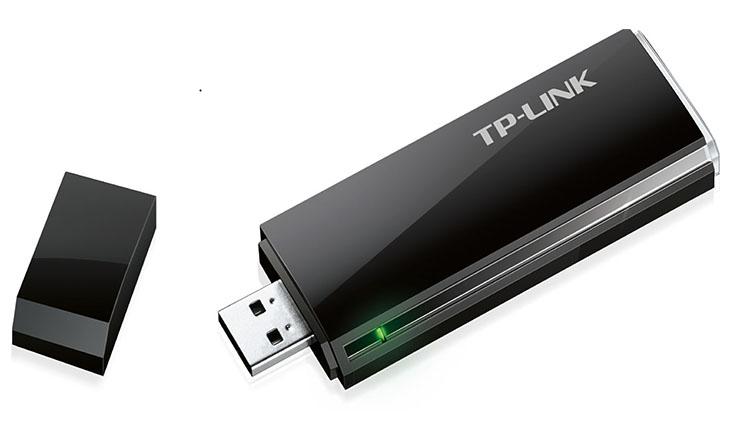
\includegraphics[width=0.6\linewidth]{Chapters/Chapter2/Figures/wifi_adapter.png}
		\caption{TP-Link Wi-Fi USB\\ Adapter N900 TL-WDN4200.}
		\label{fig:wifi_adapter}
	\end{minipage}		
	\begin{minipage}[b]{0.5\textwidth}
		\centering
		\begin{tabular}{| l | c |}
			\hline
			\textbf{Προδιαγραφές} & \textbf{TP-Link Wi-Fi USB Adapter}\\
			 &  \textbf{N900 TL-WDN4200}\\ \hline
			Σύνδεση & USB 2.0 \\ \hline
			Ταχύτητα & Dual Band $2 \times 450Mbps$\\ \hline
			Πρότυπο & IEEE 802.11b/g/n\\ \hline
			Συχνότητα & 2.4/5GHz\\ \hline
			Ασφάλεια & WEP (64-128bit)\\ \hline
		\end{tabular}
		\captionof{table}{Προδιαγραφές TP-Link Wi-Fi USB\\ Adapter N900 TL-WDN4200.}
		\label{tab:wifi_adapter_specs}
	\end{minipage}
\end{figure}


\bigskip
\subsubsection{Διασύνδεση Υποσυστημάτων}
Στις παραπάνω ενότητες, αναφέρθηκαν τα επιμέρους υποσυστήματα της ρομποτικής πλατφόρμας \textit{Monstertruck} και έγινε φανερό, ότι δεν χρησιμοποιούνται οι ίδιες διεπαφές επικοινωνίας σε κάθε συσκευή, αλλά και ότι κάθε συσκευή, χρησιμοποιεί το δικό της πρωτόκολλο επικοινωνίας. Το μόνο κοινό όλων των υποσυστημάτων, είναι η διασύνδεση και η συγκέντρωση της πληροφορίας, στον κεντρικό κόμβο του συστήματος, τον υπολογιστή \textit{Odroid-XU4}.

\bigskip
Ένα σημαντικό πρόβλημα, του υπολογιστή \textit{Odroid-XU4}, αποτελεί ο ανεπαρκής, για την συγκεκριμένη εφαρμογή, αριθμός θυρών διεπαφής σειριακής επικοινωνίας USB. Επομένως, για την ταυτόχρονη λειτουργία, όλων των επιμέρους αισθητήρων και ελεγκτών του συστήματος, κρίθηκε απαραίτητη η επέκταση του ηλεκτρονικού εξοπλισμού της ρομποτικής πλατφόρμας \textit{Monstertruck}, με την προσθήκη δύο \textit{διακλαδωτών USB (USB Hubs)}.

\bigskip
\textbf{<TODO: Add photos of USB hubs.>}

\bigskip
Η διασύνδεση των διεπαφών, όλων των επιμέρους επιμέρους υποσυστημάτων, της ρομποτικής πλατφόρμας \textit{Monstertruck}, παρουσιάζεται στο σχήμα \ref{fig:hardware_interface_diagram}.

\begin{figure}[!ht]
	\centering
	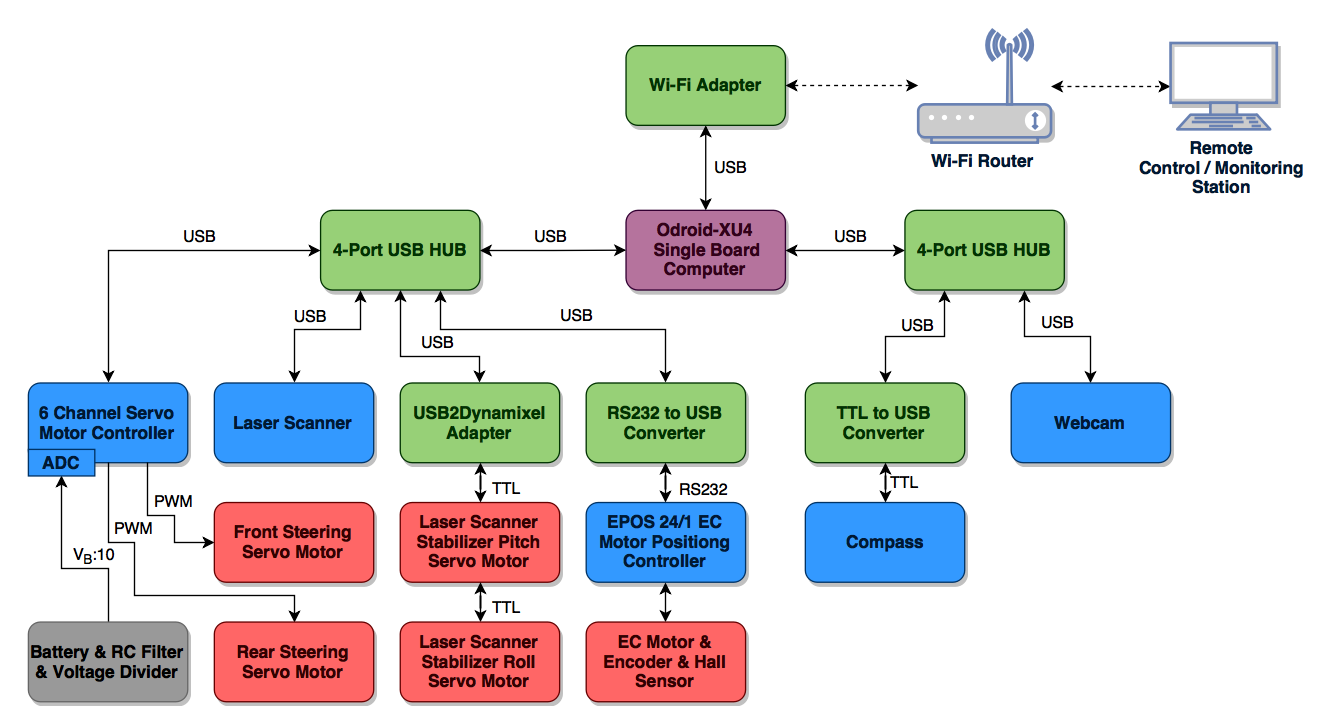
\includegraphics[width=0.9\linewidth]{Chapters/Chapter2/Figures/hardware_interface_diagram.png}
	\caption{Διασύνδεση διεπαφών των επιμέρους υποσυστημάτων της ρομποτικής πλατφόρμας \textit{Monstertruck}.}
	\label{fig:hardware_interface_diagram}
\end{figure}


\bigskip
\subsubsection{Σύστημα Τροφοδοσίας}
Από την παρουσίαση των επιμέρους υποσυστημάτων της ρομποτικής πλατφόρμας \textit{Monstertruck}, που πραγματοποιήθηκε στις προηγούμενες παραγράφους, προκύπτει, ότι, κάθε υποσύστημα - συσκευή, περιλαμβάνει διαφορετικές προδιαγραφές τροφοδοσίας. Επομένως, απαιτείται, ένα εκτενές και πλήρες σύστημα τροφοδοσίας, που να προσφέρει τις απαιτούμενες προδιαγραφές για κάθε υποσύστημα ξεχωριστά, για την ταυτόχρονη λειτουργία, όλων μαζί, αλλά και να επιτρέπει περιθώρια επέκτασης. Επίσης, θα πρέπει να περιλαμβάνει, επαρκής απομόνωση της τροφοδοσίας των ευαίσθητων ηλεκτρονικών υποσυστημάτων, από άλλα υποσυστήματα που εισάγουν θόρυβο στις γραμμές τροφοδοσίας, όπως οι κινητήρες και οι σερβοκινητήρες. 

\bigskip
Όπως, παρουσιάζεται και στο σχήμα \ref{fig:power_distribution}, ως πηγή τροφοδοσίας της ρομποτικής πλατφόρμας \textit{Monstertruck}, χρησιμοποιείται μία μπαταρία \textit{Λιθίου-Πολυμερών} (σχήμα \ref{fig:battery}) με ονομαστική τάση 22.2V, μέγιστη τάση 25.2V ($100\%$ φόρτιση) και 3700/4000/5000mAh. Η τροφοδοσία που παρέχει η μπαταρία, τροφοδοτείται σε έναν \textit{διακλαδωτή (Battery Distribution Board)}, από τον οποίο τροφοδοτούνται ο ελεγκτής \textit{EPOS 24/1} που τροφοδοτεί και τον κινητήρα του οχήματος, ο \textit{12V DC-DC μετατροπέας} και το \textit{τροφοδοτικό M4-ATX}.

\begin{figure}[!ht]
	\centering
	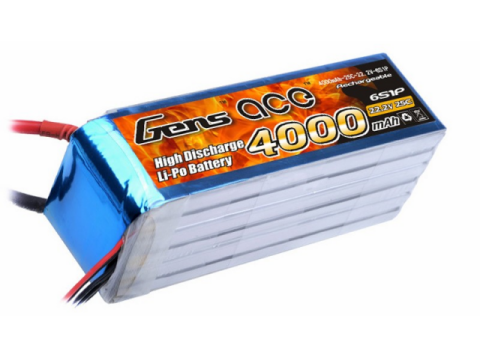
\includegraphics[width=0.3\linewidth]{Chapters/Chapter2/Figures/battery.png}
	\caption{Μπαταρία Gens ace, LiPo, 22.2V, 4000mAh.}
	\label{fig:battery}
\end{figure}

Ο \textit{12V DC-DC μετατροπέας} τροφοδοτεί με 12V, μέσω ενός \textit{διακλαδωτή (Motor Distribution Board)} τους \textit{έξυπνους σερβοκινητήρες Dynamixel}, του \textit{σταθεροποιητή Pitch-Roll} του \textit{σαρωτή λέιζερ}, όπως επίσης και έναν ανεμιστήρα, υπεύθυνο, για την ψύξη του υπολογιστή \textit{Odroid-XU4}.

\bigskip
Το τροφοδοτικό \textit{M4-ATX}, παράγει εξόδους τροφοδοσίας 5V και 12V και τροφοδοτεί την πλειονότητα των ηλεκτρονικών συστημάτων της ρομποτικής πλατφόρμας. Αρχικά, τροφοδοτεί απευθείας έναν \textit{5V DC-DC μετατροπέα}, ο οποίος χρησιμοποιείται για να τροφοδοτεί τους σερβοκινητήρες του συστήματος στρέψης - \textit{τετραδιεύθυνσης} της ρομποτικής πλατφόρμας, απομονώνοντας, ταυτόχρονα την τροφοδοσία των σερβοκινητήρων από την τροφοδοσία των υπόλοιπων ηλεκτρονικών υποσυστημάτων, που παρουσιάζουν ευαισθησία στον θόρυβο. Τα υπόλοιπα ηλεκτρονικά υποσυστήματα της ρομποτικής πλατφόρμας, τροφοδοτούνται, από το τροφοδοτικό \textit{M4-ATX}, μέσω ενός \textit{διακλαδωτή (Electronics Distribution Board)}, είτε άμεσα, όπως ο υπολογιστής \textit{Odroid-XU4}, ο \textit{σαρωτής λέιζερ} και οι \textit{διακλαδωτές USB (USB Hubs)}, είτε μέσω του υπολογιστή και των \textit{διακλαδωτών USB}.

\begin{figure}[!ht]
	\centering
	\subfloat[Τροφοτικό M4-ATX.]{
		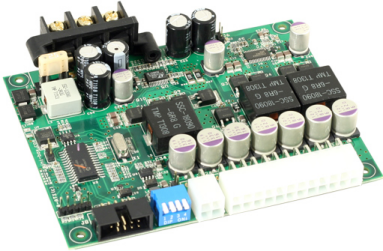
\includegraphics[width=0.32\linewidth]{Chapters/Chapter2/Figures/m4atx.png}
		\label{fig:m4atx}}
	\subfloat[5V DC-DC Μετατροπέας.]{
		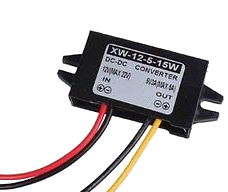
\includegraphics[width=0.32\linewidth]{Chapters/Chapter2/Figures/5v_dc_dc_converter.png}
		\label{fig:5v_dc_dc_converter}}
	\subfloat[12V DC-DC Μετατροπέας.]{
		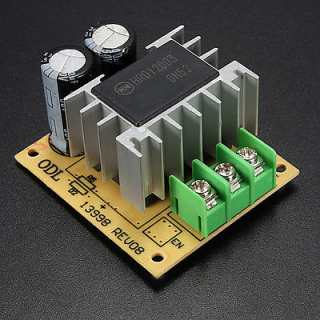
\includegraphics[width=0.32\linewidth]{Chapters/Chapter2/Figures/12v_dc_dc_converter.png}
		\label{fig:12v_dc_dc_converter}}
	\caption{Επιμέρους τμήματα συστήματος τροφοδοσίας.}
\end{figure}

% TODO
\bigskip
\begin{center}
\textbf{<TODO: Insert distribution boards>}
\end{center}

\bigskip
\begin{figure}[!ht]
	\centering
	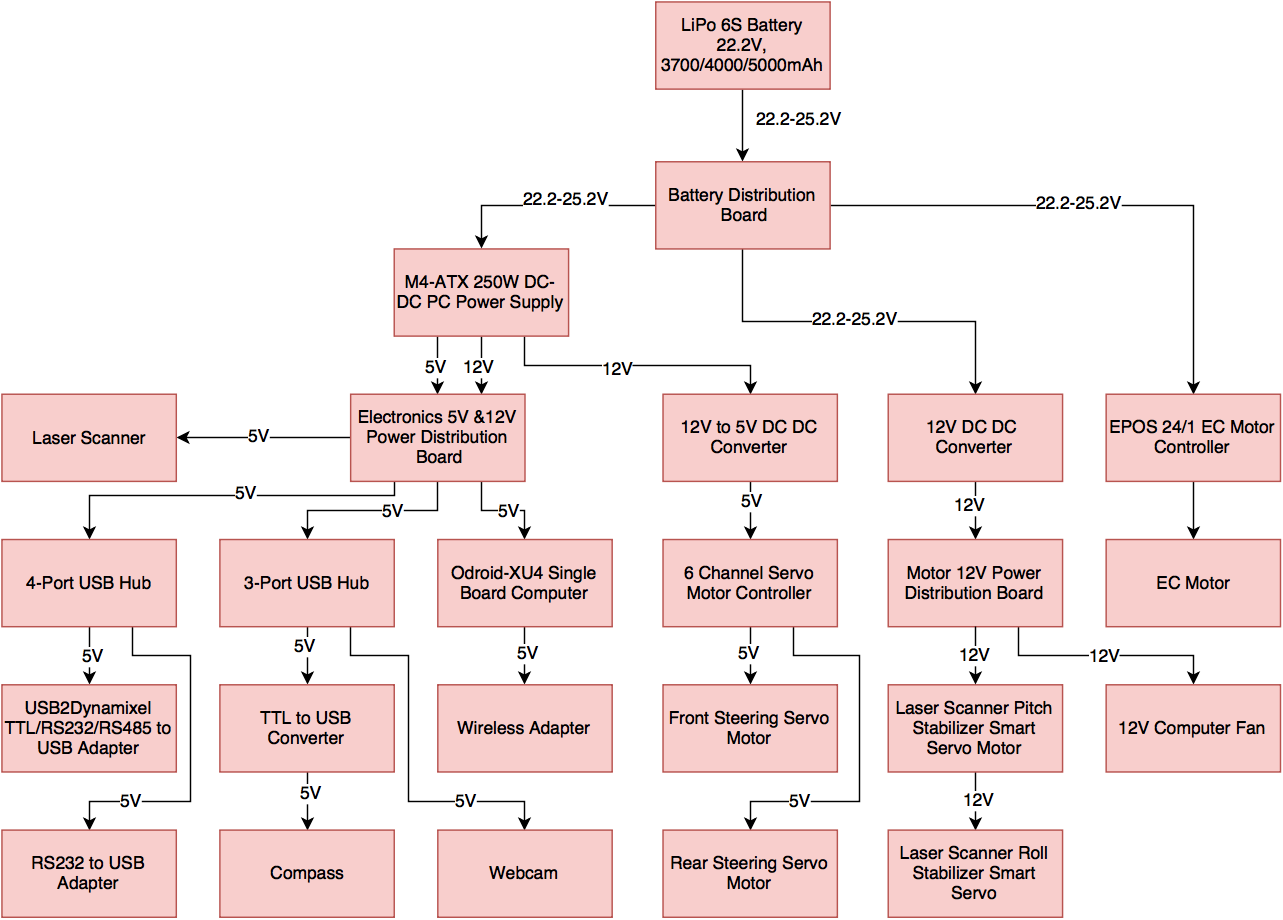
\includegraphics[width=0.8\linewidth]{Chapters/Chapter2/Figures/power_distribution.png}
	\caption{Σύστημα Τροφοδοσίας των επιμέρους υποσυστημάτων της ρομποτικής πλατφόρμας \textit{Monstertruck}.}
	\label{fig:power_distribution}
\end{figure}


%%%%%%%%%%%%%%%%%%%%%%%%%%%%%%%%%%%%%%%%%%%%%%%%%%%%%%%%%%%%%%%%%%%%%%%%%%%%%%%%%%%%%%%%%%%%
%\bigskip
%\subsubsection{Χωροθέτηση Υποσυστημάτων Ρομποτικής Πλατφόρμας \textit{Monstertruck}} ???
%%%%%%%%%%%%%%%%%%%%%%%%%%%%%%%%%%%%%%%%%%%%%%%%%%%%%%%%%%%%%%%%%%%%%%%%%%%%%%%%%%%%%%%%%%%%

%----------------------------------------------------------------------------------------
%	SECTION 1: Motion Transfer System
%----------------------------------------------------------------------------------------
\newpage
\section{Σύστημα Μετάδοσης Κίνησης}
Ένα αυτοκίνητο όχημα, για να κινηθεί, απαιτεί την ύπαρξη \textit{ενεργοποιητών(actuators)}, οι οποίοι μετατρέπουν την ενέργεια από μία πηγή τροφοδοσίας και ένα σήμα ελέγχου σε μηχανική κίνηση. Τον σκοπό αυτό, εξυπηρετούν οι κινητήρες και στην προκειμένη περίπτωση, για την επίτευξη της μηχανικής κίνησης του υλοποιημένου ρομποτικού οχήματος, χρησιμοποιούνται ένας κινητήρας, ο οποίος, μέσω ενός συστήματος μετάδοσης κίνησης, μεταδίδει την περιστροφική κίνηση του και στους τέσσερις τροχούς του οχήματος (\textit{τετρακίνηση}) και δύο σερβοκινητήρες, οι οποίοι στρίβουν και τους τέσσερις τροχούς, με ανεξάρτητη στρέψη των μπροστινών, από τους πίσω τροχούς  (\textit{τετραδιεύθυνση}). Στην συνέχεια, παρουσιάζεται η ανάλυση των μηχανισμών \textit{τετρακίνησης} και \textit{τετραδιεύθυνσης} της ρομποτικής πλατφόρμας \textit{Monstertruck}.


\bigskip
\subsection{Σύστημα Τετρακίνησης}
Η μετάδοση της κίνησης, από τον μοναδικό κινητήρα του οχήματος, προς τους τέσσερις τροχούς, δηλαδή η τετρακίνηση επιτυγχάνεται, μέσω του \textit{συστήματος μετάδοσης κίνησης (drivetrain)}, όπως φαίνεται στο σχήμα \ref{fig:drivetrain}. Το σύστημα αυτό περιλαμβάνει, συνολικά τέσσερα στάδια μετάδοσης της περιστροφικής κίνησης του κινητήρα, προς κάθε τροχό, όπου κάθε στάδιο εισάγει ένα λόγο μείωσης των στροφών, αλλά ταυτόχρονα, αντίστοιχο λόγο αύξησης της ροπής στρέψης.

\bigskip
\begin{figure}[!ht]
	\centering
	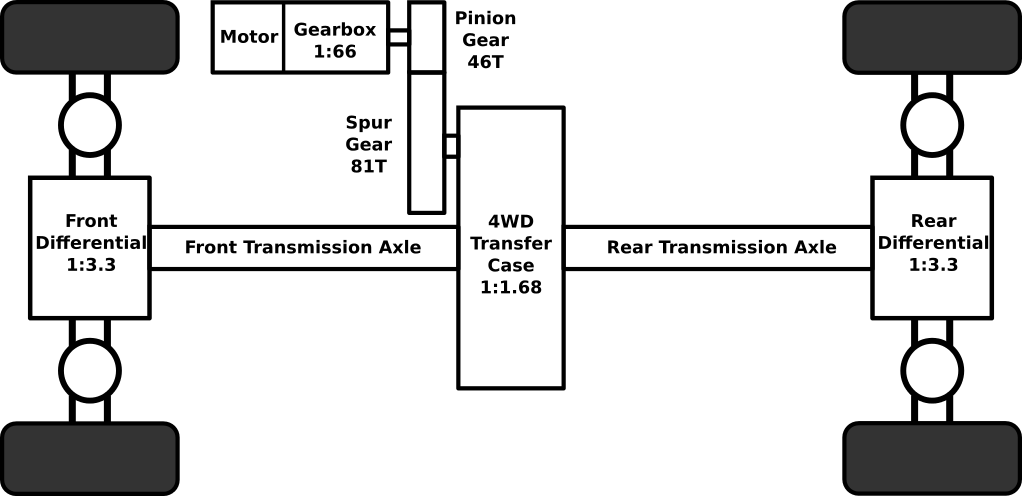
\includegraphics[width=0.8\linewidth]{Chapters/Chapter2/Figures/drivetrain.png}
	\caption{Σύστημα Μετάδοσης Κίνησης (Drivetrain) της ρομποτικής πλατφόρμας \textit{Monstertruck}}.
	\label{fig:drivetrain}
\end{figure}

\bigskip
Το πρώτο στάδιο, αποτελεί το \textit{κιβώτιο ταχυτήτων - μειωτήρας (gearbox)} του κινητήρα, το οποίο περιγράφεται από ένα λόγο μετάδοσης $1:66$. Ο λόγος, αυτός, μειώνει την μέγιστη περιστροφική ταχύτητα του κινητήρα, από $18\,000rpm$ σε $18\,000:66=272.72rpm$.

\bigskip
Το δεύτερο στάδιο μετάδοσης, αποτελείται από δύο γρανάζια, το \textit{Πινιόν (Pinion Gear)} και \textit{Ώθησης (Spur Gear)}. Το \textit{γρανάζι Πινιόν}, μεταδίδει την κίνηση από τον κινητήρα στο \textit{γρανάζι Ώθησης}, το οποίο, με τη σειρά του μεταδίδει την κίνηση στο επόμενο στάδιο μετάδοσης. Το \textit{γρανάζι Πινιόν} περιλαμβάνει $46$ οδοντώσεις, ενώ το \textit{γρανάζι Ώθησης}, $84$, έχοντας ως αποτέλεσμα ένα λόγο μετάδοσης $46:81=1:1.76$. Με την μείωση του δεύτερου σταδίου, η μέγιστη ταχύτητα μειώνεται στα $272.72:1.76 = 154.96rpm$.

\begin{figure}[!ht]
	\centering
	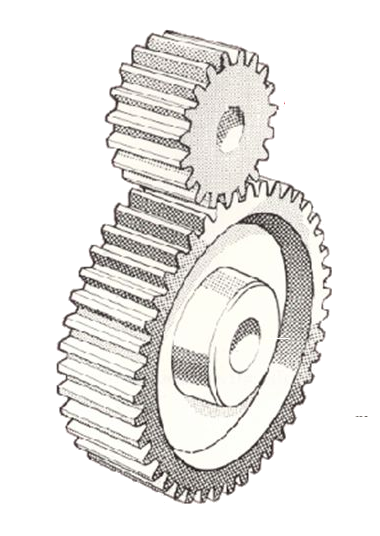
\includegraphics[width=0.2\linewidth]{Chapters/Chapter2/Figures/spur_pinion_gears.png}
	\caption{Γρανάζια Πινιόν και Ώθησης.}
	\label{fig:spur_pinion_gears}
\end{figure}

\bigskip
Το τρίτο στάδιο μετάδοσης και σημαντικότερο, για την επίτευξη \textit{τετρακίνησης}, περιλαμβάνει το \textit{κιβώτιο μετάδοσης (Transfer Case)} του μπροστινού και του πίσω άξονα, που φαίνεται στο σχήμα \ref{fig:transfer_case}. Το \textit{κιβώτιο μετάδοσης}, περιλαμβάνει δύο γρανάζια, το \textit{γρανάζι μετάδοσης (Transmission Gear)} και το \textit{διαφορικό γρανάζι (Differential Gear)}. Η περιστροφική κίνηση μεταδίδεται, από το \textit{γρανάζι Ώθησης}, προς το \textit{γρανάζι μετάδοσης}, μέσω ενός μηχανισμού \textit{σφιγκτήρα ολίσθησης (slipper clutch)}, που επιτρέπει την αποσύμπλεξη των γραναζιών, μέσω ολίσθησης, σε περίπτωση, υψηλής ροπής στους τροχούς, που θα μπορούσαν να προκαλέσουν ζημιά στα γρανάζια και στους άξονες μετάδοσης. Υπό φυσιολογικές συνθήκες, το \textit{γρανάζι μετάδοσης}, μεταδίδει την περιστροφική κίνηση προς το \textit{διαφορικό γρανάζι} και έπειτα προς τους δύο άξονες μετάδοσης, με λόγο μετάδοσης $1:1.68$. Επομένως, έχουμε μία επιπλέον μείωση των στροφών, με αποτέλεσμα $154.96:1.68=92.24rpm$.

\begin{figure}[!ht]
	\centering
	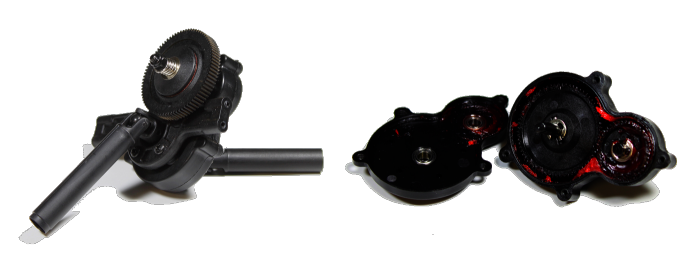
\includegraphics[width=0.8\linewidth]{Chapters/Chapter2/Figures/transfer_case.png}
	\caption{To κιβώτιο μετάδοσης κίνησης (Transfer Case) του οχήματος GroundPounder.}
	\label{fig:transfer_case}
\end{figure}

\bigskip
Το τέταρτο και τελευταίο στάδιο μετάδοσης της κίνησης, αποτελείται από δύο \textit{διαφορικά (differential)}, ένα για τους μπροστινούς τροχούς και ένα για τους πίσω. Το \textit{διαφορικό} είναι ένας μηχανισμός, ο οποίος μετατρέπει την κατεύθυνση κίνησης, από την ευθύγραμμη, του άξονα μετάδοσης, στην εγκάρσια, των ημιαξόνων κάθε τροχού. Παράλληλα, επιτρέπει σε δύο τροχούς, έναν αριστερό και ένα δεξιό, να κινούνται με διαφορετική περιστροφική ταχύτητα, ανάλογα με την πρόσφυση σε κάθε έναν, από αυτούς. Ο μηχανισμός, αυτός, είναι απαραίτητος, καθώς, όταν ένα όχημα προσπαθεί να στρίψει, ακολουθώντας μία καμπύλη, οι τροχοί που βρίσκονται στην εξωτερική πλευρά της καμπύλης, διανύουν μεγαλύτερη απόσταση, από τους εσωτερικούς τροχούς και άρα θα πρέπει να κινούνται με μεγαλύτερη ταχύτητα. Τέλος, το κάθε \textit{διαφορικό} εισάγει, ακόμη, έναν τελευταίο λόγο μείωσης των στροφών, της τάξης του $1:3.3$, οπότε η τελική μέγιστη ταχύτητα περιστροφής των τροχών προκύπτει $92.24:3.3=27.95rpm$.

\begin{figure}[!ht]
	\begin{minipage}{.49\textwidth}
		\centering
		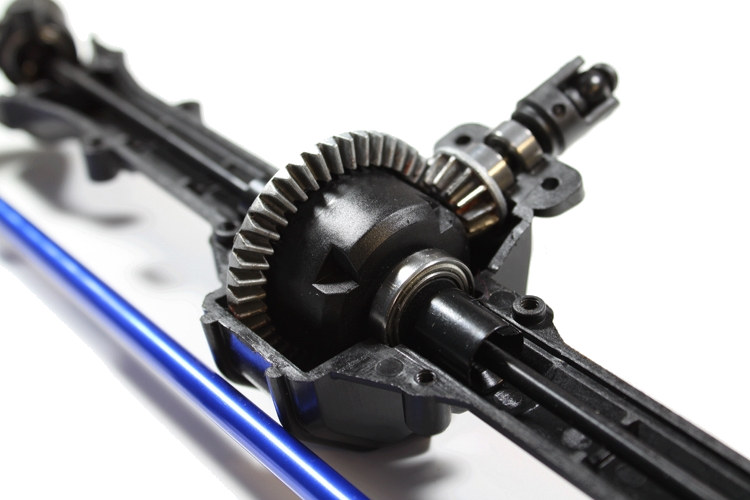
\includegraphics[width=0.5\linewidth]{Chapters/Chapter2/Figures/differential.png}
		\captionof{figure}{Το διαφορικό (Differential) του οχήματος GroundPounder.}
		\label{fig:differential}
	\end{minipage}
	\begin{minipage}{.5\textwidth}
	 	\centering		
		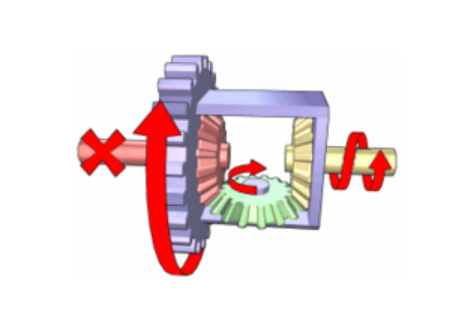
\includegraphics[width=0.5\linewidth]		
			{Chapters/Chapter2/Figures/differential_function.png}
		\captionof{figure}{Λειτουργία ενδεικτικού μηχανισμού διαφορικού.}
		\label{fig:differential_function}
	\end{minipage}
\end{figure}

\bigskip
Επομένως, η σχέση μετάδοσης της περιστροφικής ταχύτητας, από τον κινητήρα, στους τροχούς προκύπτει:

\begin{equation}
	\omega_{wheel} = \omega_{motor} / (\lambda_{gearbox} \times \lambda_{spur\_pinion} \times \lambda_{transfer\_case} \times \lambda_{differential}) = \omega_{motor} / 644
\end{equation}

\bigskip
\subsection{Σύστημα Τετραδιεύθυνσης}
Η ρομποτική πλατφόρμα \textit{Monstertruck}, περιλαμβάνει δύο σερβοκινητήρες, υπεύθυνους για την ανεξάρτητη στρέψη των μπροστινών και πίσω τροχών. Η ανεξάρτητη αυτή στρέψη, επιτρέπει στο όχημα να λειτουργεί με \textit{μπροστινή στρέψη (FWS)}, \textit{πίσω στρέψη (RWS)}, ή \textit{ταυτόχρονη στρέψη (τετραδιεύθυνση - 4WS)} των τροχών. Στην ταυτόχρονη στρέψη, οι μπροστινοί τροχοί, μπορεί να στρίβουν, είτε, με την ίδια φορά \textit{(Crab Steering)}, είτε με αντίθετη \textit{(Counter Steering)}, από τους πίσω.

\bigskip
Εφόσον, υπάρχει ένας σερβοκινητήρας, για τους μπροστινούς τροχούς και ένας για τους πίσω, γεννάται το ερώτημα, πώς μεταδίδεται η στρέψη από έναν σερβοκινητήρα σε δύο τροχούς, έναν αριστερό και έναν δεξιό τροχό. Ο μηχανισμός, που λύνει το πρόβλημα, στην προκειμένη περίπτωση, ονομάζεται \textit{Μηχανισμός Στρέψης, μέσω Συνδέσμου Έλξης (Drag Link Steering Mechanism)}. Ο  μηχανισμός στρέψης του οχήματος GroundPounder αποτελείται από έναν σερβοκινητήρα, ένα \textit{μπράτσο Pitman (Pitman Arm)}, έναν \textit{σύνδεσμο έλξης (Drag Link)} και έναν \textit{σύνδεσμο ένωσης των τροχών (Tie Rod)}, όπως επίσης και τις \textit{αρθρώσεις στρέψης των τροχών (Wheel Steering Knuckles)}.

\begin{figure}[!ht]
	\centering
	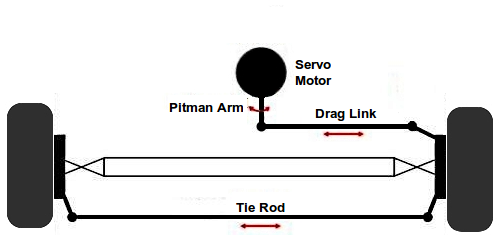
\includegraphics[width=0.6\linewidth]{Chapters/Chapter2/Figures/my_drag_link_steering.png}
	\caption{Μηχανισμός στρέψης, με άξονα έλξης (Drag Link Steering Mechanism).}
	\label{fig:drag_link_steering}
\end{figure}

\bigskip
Η περιστροφική κίνηση του σερβοκινητήρα, μεταδίδεται μέσω του \textit{μπράτσου Pitman} και μετατρέπεται σε μεταφορική κίνηση του \textit{συνδέσμου έλξης}, η οποία με τη σειρά της μετατρέπεται σε στρέψη της άρθρωσης του δεξιού τροχού. Η στρέψη, τώρα, της δεξιάς άρθρωσης, παρασύρει τον \textit{σύνδεσμο ένωσης} των αρθρώσεων στρέψης των τροχών σε μεταφορική κίνηση, η οποία, έχει σαν αποτέλεσμα την στρέψη και του αριστερού τροχού. Ακολούθως, αναλύεται η λειτουργία του μηχανισμού στρέψης, σε δύο βήματα. Πρώτα υπολογίζεται η μετατόπιση $\Delta x$ του \textit{συνδέσμου έλξης}, συναρτήσει της γωνίας στρέψης $\theta$ του σερβοκινητήρα και έπειτα, συναρτήσει της γωνίας στρέψης $\delta$ της άρθρωσης τροχού, με την οποία, είναι συνδεδεμένος ο \textit{σύνδεσμος έλξης}.

\bigskip
\begin{figure}[!ht]
	\centering
	\subfloat[Ανάλυση για $\theta < 0$.]{
	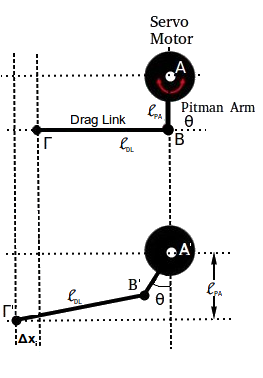
\includegraphics[width=0.4\linewidth]{Chapters/Chapter2/Figures/drag_link_analysis_1.png}
	\label{fig:drag_link_analysis_a}}
	\centering
	\subfloat[Ανάλυση για $\theta > 0$.]{
	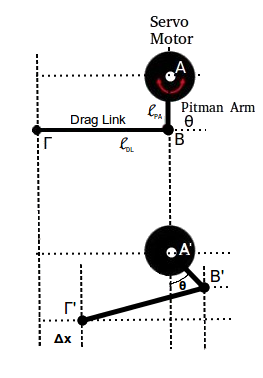
\includegraphics[width=0.4\linewidth]{Chapters/Chapter2/Figures/drag_link_analysis_2.png}
	\label{fig:drag_link_analysis_b}}
	\caption{Μετάδοση κίνησης από τον σερβοκινητήρα και το μπράτσο Pitman στον σύνδεσμο έλξης.}
	\label{fig:drag_link_analysis}	
\end{figure}

\bigskip
Λαμβάνοντας την παραδοχή, ότι η άκρη (σημείο Γ) του συνδέσμου έλξης, κινείται, μόνο οριζόντια και όχι κάθετα και με βάση το σχήμα \ref{fig:drag_link_analysis} και απλή γεωμετρική ανάλυση, μπορεί να εξαχθεί η  σχέση μεταξύ της γωνίας στρέψης $\theta$ του σερβοκινητήρα και της μετατόπισης $\Delta x$ του \textit{συνδέσμου έλξης}, ως:

\begin{equation}
	\label{eq:drag_link_displacement}
	\Delta x =
	\begin{cases}
		\sqrt{l_{DL}^2 - l_{PA}^2(1-\cos(\theta))^2} + l_{PA} \sin(|\theta|) - l_{DL},  &\theta < 0\\ \\
	0, &\theta = 0\\ \\ 
	-\sqrt{l_{DL}^2 - l_{PA}^2(1-\cos(\theta))^2} - l_{PA} \sin(|\theta|) - l_{DL}, &\theta > 0
	\end{cases}
\end{equation}

\bigskip\noindent
όπου $l_{DL}$ είναι το μήκος του \textit{συνδέσμου έλξης} και $l_{PA}$ είναι το μήκος του \textit{μπράτσου Pitman}.

\begin{figure}[!ht]
	\centering
	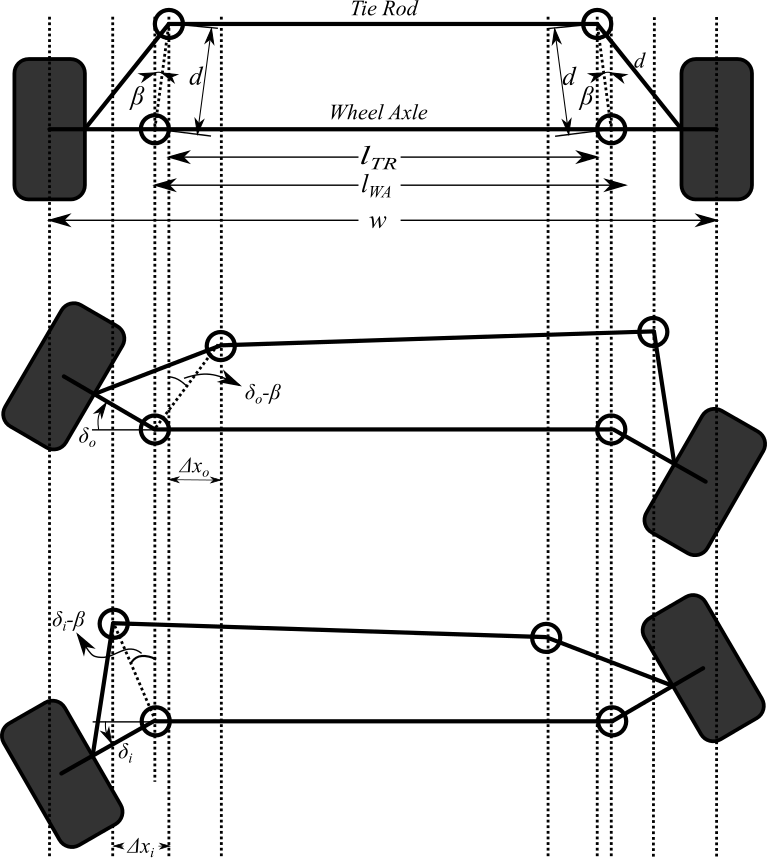
\includegraphics[width=0.8\linewidth]{Chapters/Chapter2/Figures/trapezoid_steering_mechanism.png}
	\caption{Τραπεζοειδής Μηχανισμός στρέψης των τροχών.}
	\label{fig:trapezoid_steering_mechanism}
\end{figure}

\bigskip
Με βάση το σχήμα \ref{fig:trapezoid_steering_mechanism}, μέσω γεωμετρικής ανάλυσης, προκύπτει ότι, η μετατόπιση του σύνδεσμου έλξης $\Delta x$, συναρτήσει της γωνίας στρέψης, του συνδεδεμένου τροχού, αριστερού, στην προκειμένη περίπτωση, για τις περιπτώσεις, ο τροχός να είναι στην εσωτερική ή στην εξωτερική  πλευρά της στροφής, προκύπτει:
 
\begin{equation}
\label{eq:tie_rod_inner_displacement}
	\Delta x_i = d \sin(\delta_i - \beta) + d \sin(\beta)
\end{equation}

\begin{equation}
	\label{eq:tie_rod_outer_displacement}
	\Delta x_o = d \sin(\delta_o + \beta) - d \sin(\beta)
\end{equation}

\bigskip
Εξισώνοντας, τώρα, τις σχέσεις (\ref{eq:drag_link_displacement}), (\ref{eq:tie_rod_inner_displacement}), (\ref{eq:tie_rod_outer_displacement}), προκύπτει η σχέση μεταξύ της γωνίας στρέψης του σερβοκινητήρα και της γωνίας στρέψης του αριστερού τροχού, για τις περιπτώσεις που είναι εσωτερικά ($\delta_i$) στην στροφή και εξωτερικά ($\delta_o$):

\begin{equation}
	\label{eq:inner_steering_angle}
	\delta_i = \beta + \sin^{-1}{ \Bigg(
		\frac{
		\sqrt{l_{DL}^2 - l_{PA}^2(1-\cos(\theta))} + l_{PA} \sin{|\theta|} - l_{DL} - d \sin{\beta}}{d}} \Bigg)
\end{equation}

\begin{equation}
	\label{eq:outer_steering_angle}
	\delta_o = -\beta + \sin^{-1}{ \Bigg(
		\frac{
		-\sqrt{l_{DL}^2 - l_{PA}^2(1-\cos(\theta))} - l_{PA} \sin{|\theta|} - l_{DL} + d \sin{\beta}}{d}} \Bigg)
\end{equation}

\bigskip
Ο υπολογισμός της γωνίας στρέψης, του απέναντι τροχού, δηλαδή, στην προκειμένη περίπτωση, του δεξιού τροχού, προκύπτει από τις εξισώσεις \textit{τραπεζοειδούς μηχανισμού στρέψης τροχών} \cite{vehicle_dynamics}, προσαρμοσμένες στην παρούσα τοπολογία:

\begin{equation}
	\label{eq:trapezoid_steering_mechanism}
	sin(\beta + \delta_o) + sin(\beta - \delta_i) = \frac{L}{d} + \sqrt{\big(\frac{L}{d} - w \sin{\beta} \big)^2 - \big(\cos{(\beta-\delta_i)} - \cos{(\beta+\delta_o)}\big)^2}
\end{equation}

\bigskip
Αντικαθιστώντας την τιμή για την $\delta_i$, στην εξίσωση (\ref{eq:trapezoid_steering_mechanism}) θα πρέπει να εφαρμοστεί, ένας επαναληπτικός αλγόριθμος, για την εύρεση της $\delta_o$ και αντίστροφα.

\bigskip
Για την απλοποίηση της όλης διαδικασίας μετατροπής της γωνίας στρέψης του σερβοκινητήρα, σε γωνίες στρέψης των τροχών και αντίστροφα, χρησιμοποιήθηκαν πολυωνυμικές προσεγγίσεις των σχέσεων μεταξύ αυτών, λύνοντας, επαναληπτικά και για όλες τις δυνατές τιμές, τις εξισώσεις (\ref{eq:inner_steering_angle}), (\ref{eq:outer_steering_angle}), (\ref{eq:trapezoid_steering_mechanism}).

\begin{align}
\begin{split}
	\delta_{LF} &= -0.0082 \theta_{F}^5 - 0.0162 \theta_{F}^4 - 0.00605 \theta_{F}^3 - 0.0192 \theta_{F}^2 + 0.6691 \theta_{F}\\
	\delta_{LR} &= 0.0082 \theta_{R}^5 + 0.0162 \theta_{R}^4 + 0.00605 \theta_{R}^3 + 0.0192 \theta_{R}^2 - 0.6691 \theta_{R}\\
	\delta_{RF} &= 0.0126 \delta_{LF}^5 - 0.0432 \delta_{LF}^4 + 0.0067 \delta_{LF}^3 - 0.0851 \delta_{LF}^2 + 0.9997 \delta_{LF} + 0.0035\\
	\delta_{RR} &= -0.0126 \delta_{LR}^5 + 0.0432 \delta_{LR}^4 - 0.0067 \delta_{LR}^3 + 0.0851 \delta_{LR}^2 - 0.9997 \delta_{LR} - 0.0035\\
	\theta_{F} &= 0.5334 \delta_{LF}^5 + 0.2997 \delta_{LF}^4 + 0.2857 \delta_{LF}^3 + 0.0556 \delta_{LF}^2 + 1.4951 \delta_{LF}\\
	\theta_{R} &= - 0.5334 \delta_{LR}^5 - 0.2997 \delta_{LR}^4 - 0.2857 \delta_{LR}^3 - 0.0556 \delta_{LR}^2 - 1.4951 \delta_{LR}\\
\end{split}
\end{align}

όπου:

\begin{description}
	\item[\theta_{F}] είναι η γωνία στρέψης του μπροστινού σερβοκινητήρα
	\item[\theta_{R}] είναι η γωνία στρέψης του πίσω σερβοκινητήρα
	\item[\delta_{LF}] είναι η γωνία στρέψης του μπροστινού αριστερού τροχού
	\item[\delta_{RF}] είναι η γωνία στρέψης του μπροστινού δεξιού τροχού
	\item[\delta_{LR}] είναι η γωνία στρέψης του πίσω αριστερού τροχού
	\item[\delta_{RR}] είναι η γωνία στρέψης του πίσω δεξιού τροχού
\end{description}


%----------------------------------------------------------------------------------------
%	SECTION 3: Kinematic Analysis
%----------------------------------------------------------------------------------------
\section{Κινηματική Ανάλυση}
Ένα σύγχρονο αυτοκίνητο όχημα, στην πλειονότητα των περιπτώσεων, για να κινηθεί, περιλαμβάνει έναν κινητήρα, ο οποίος είναι υπεύθυνος για την περιστροφική κίνηση των μπροστινών (μπροστινοκίνηση), πίσω (πισωκίνηση) ή όλων (τετρακίνηση) των τροχών. Επίσης, περιλαμβάνει ένα σύστημα στρέψης των τροχών, είτε μπροστινών (μπροστινοδιεύθυνση), είτε πισινών (πισωδιεύθυνση), είτε και των τεσσάρων (τετραδιεύθυνση), έτσι ώστε να μπορεί να εκτελεί στροφές και να μην κινείται μόνο ευθύγραμμα.

\bigskip
Μέσω της κινηματικής ανάλυσης, ενός τροχοφόρου οχήματος, γίνεται η προσπάθεια να μεταφραστούν οι κινήσεις των τροχών σε κινήσεις του οχήματος, για την περίπτωση της ευθείας κινηματικής ανάλυσης. Αντίθετα, στην αντίστροφη κινηματική ανάλυση, γίνεται προσπάθεια να μεταφραστούν οι κινήσεις του οχήματος σε κινήσεις των τροχών του.

\subsection{Κινηματικό Ackermann}
Τα συμβατικά αυτοκίνητα, που κυκλοφορούν τις τελευταίες δεκαετίες χρησιμοποιούν το λεγόμενο κινηματικό Ackermann. Το κινηματικό Ackermann, ορίζει μία συνθήκη, την λεγόμενη συνθήκη Ackermann, μεταξύ των τροχών στρέψης ενός αυτοκινήτου, που αν ικανοποιείται προβλέπει την κίνηση των τροχών, χωρίς ολίσθηση, σε χαμηλές ταχύτητες, όπου δεν λαμβάνουν χώρα δυναμικά φαινόμενα.










\subsection{Κινηματικό 4WS}
\subsection{Κινηματική Ανάλυση Οχήματος \textit{Monstertruck}}
\subsection{Μοντέλο Προσομοίωσης}